\section{Utility Evaluation Logistics}
  Detailed procedures for (deep) hedging evaluation, including
  dataset splits, model architectures, training hyperparameters,
  and evaluation metrics.

  \subsection{Hedging Tasks Specifications}
    We consider the hedging of a European call option on a single
    underlying asset \( S_t \) with strike price \( K \) and
    maturity \( T \). The option payoff at maturity is given by
    \( g(S_T) = \max(S_T - K, 0) \).

    For each sequence length tested in §\ref{sec:sequence_length},
    we have set the corresponding option maturity \( T \) to match
    the length of the generated sequences. For example, if the
    sequence length is 60 minutes, then the option maturity \( T \)
    is set to 60 minutes.

  \subsection{Algorithm Comparison Models}\label{appendix:deep-hedger-algorithms}
    In §\ref{sec:algorithm-comparison}, we described the procedure
    for comparing multiple (deep) hedger algorithms to evaluate the
    relative performance preservation on synthetic data versus real
    data.
  
      We have considered the following deep hedger algorithms:
      \begin{enumerate}[label=\textbf{[H\arabic*]}]
        \item \label{hedger:feedforwardlag} \textbf{Feedforward Layers
        Neural 
        Network (FLNN).} A standard multi-layer perceptron with 
        fully connected layers, ReLU activations, and dropout for 
        regularization.

        \item \label{hedger:feedforward} \textbf{Feedforward Time
        Neural Network (FTNN).} A feed-forward neural network designed 
          to process time series data by accepting lagged observations 
          as input features. This architecture uses fully connected 
          layers with ReLU activations and dropout for regularization, 
          enabling it to learn non-linear relationships between past 
          and future values without explicit recurrence.
        
        \item \label{hedger:lstm} \textbf{Long Short-Term Memory 
        (LSTM).} A recurrent neural network architecture designed 
        to capture temporal dependencies in sequential data, 
        particularly effective for time series tasks.
        
        \item \label{hedger:rnn} \textbf{Recurrent Neural Network (RNN).}
        An attention-based architecture that models long-range 
        dependencies in sequences without relying on recurrence, 
        utilizing self-attention mechanisms to enhance performance 
        on sequential data.
      
      \end{enumerate}
    
    We also considered the following (non-deep) hedging models:
    \begin{enumerate}[label=\textbf{[H\arabic*]}, resume]
      \item \label{hedger:black-scholes} \textbf{Black-Scholes 
      Delta Hedging (BSD).} A classical hedging strategy based on the 
      Black-Scholes option pricing model, which computes the 
      delta of the option to determine the optimal hedge ratio.

      \item \label{hedger:binomial} \textbf{Binomial Delta-Gamma Hedging (BDG).}
      A discrete-time hedging strategy that uses a binomial tree
      model to compute both delta and gamma of the option, allowing
      for more accurate hedging in the presence of non-linear price
      movements.

      \item \label{hedger:lreg} \textbf{Linear Regression Hedging (LR).} 
      A hedging strategy that uses linear regression to estimate 
      the hedge ratios based on historical data.

      \item \label{hedger:xgboost} \textbf{XGBoost Hedging (XGB).}
      A machine learning-based hedging strategy that employs
      gradient boosting decision trees to learn optimal hedge ratios
      from historical data.  
    \end{enumerate}

\begin{figure*}[h]
  \centering
  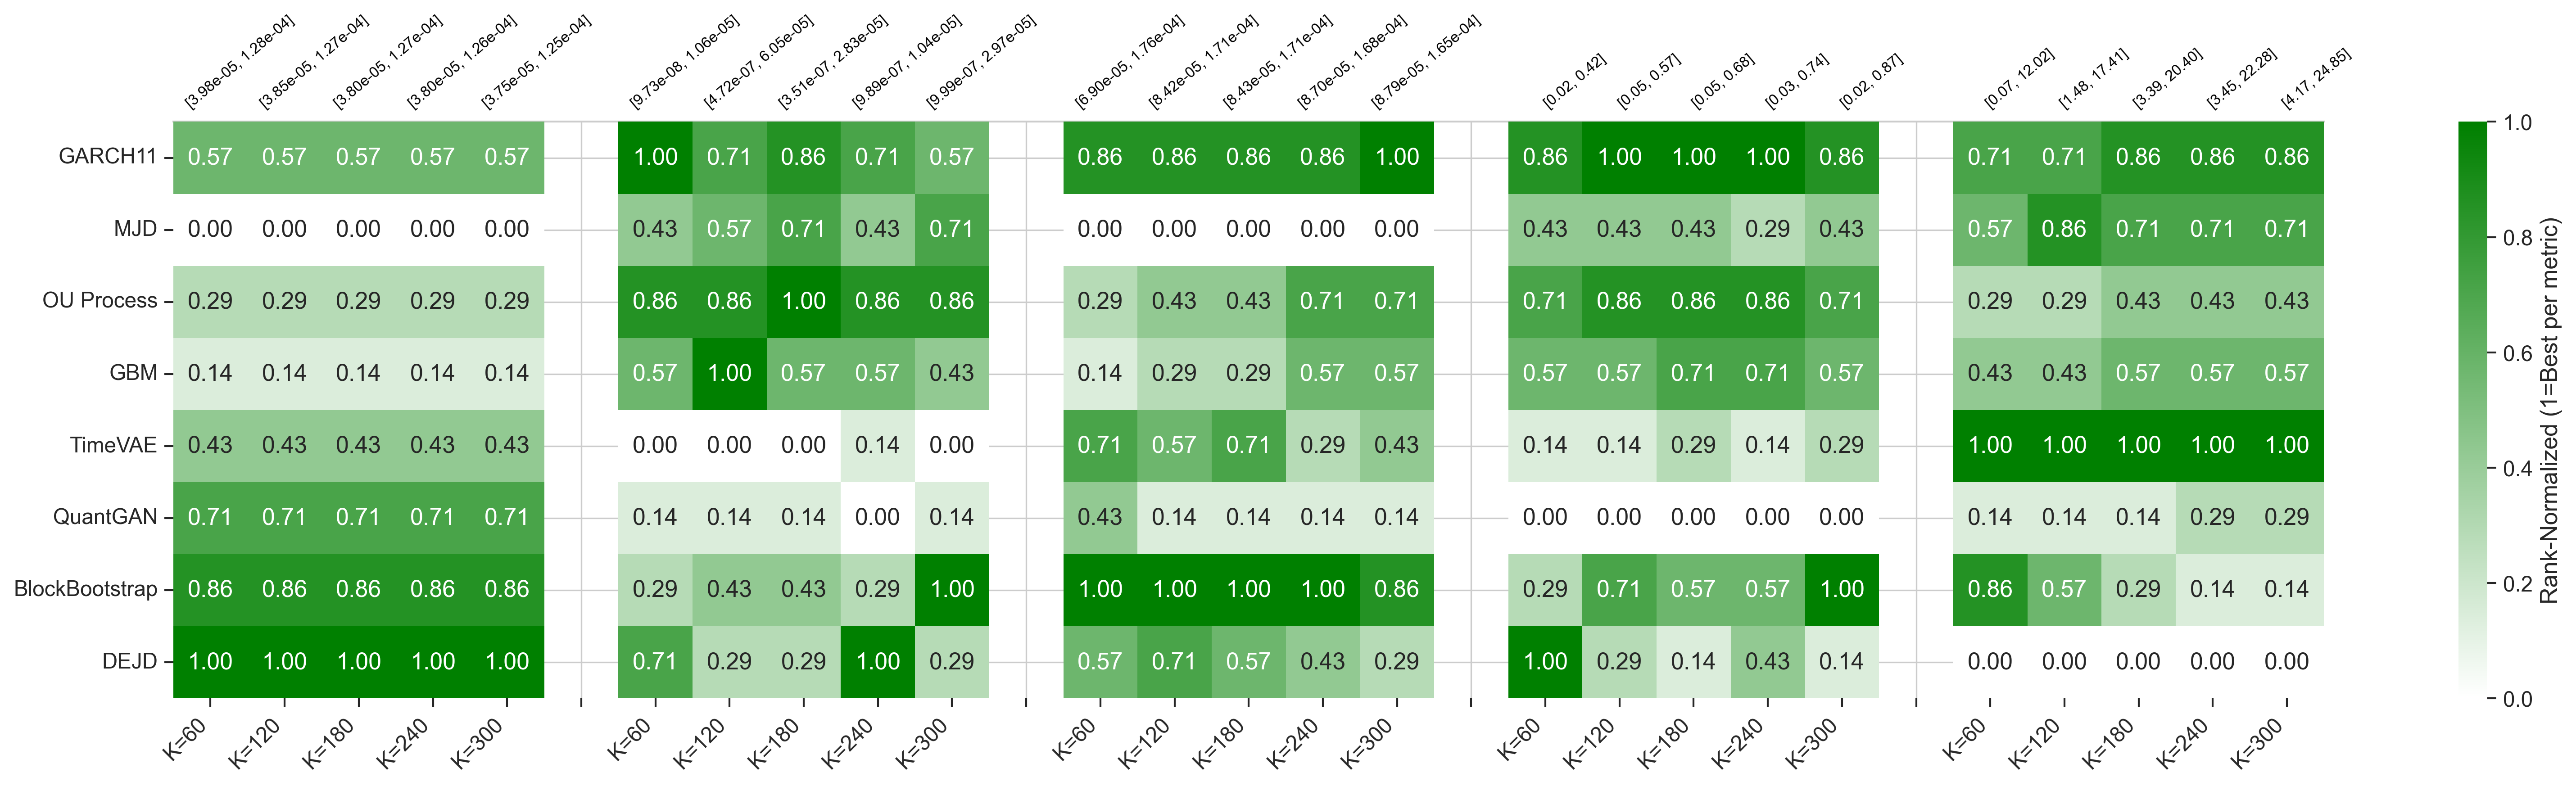
\includegraphics[width=0.9\textwidth,keepaspectratio]
  {../../results/ablation_studies/figure_3_metric_heatmaps_per_metric/figure_3_fidelity_per_metric_ranknorm.png}
  \caption{Ablation study: fidelity per-metric rank-normalized heatmap across sequence lengths.}
  \Description{Heatmap showing fidelity metrics across sequence length ablations.}
  \label{fig:ablation_fidelity}
\end{figure*}

\begin{figure*}[h]
  \centering
  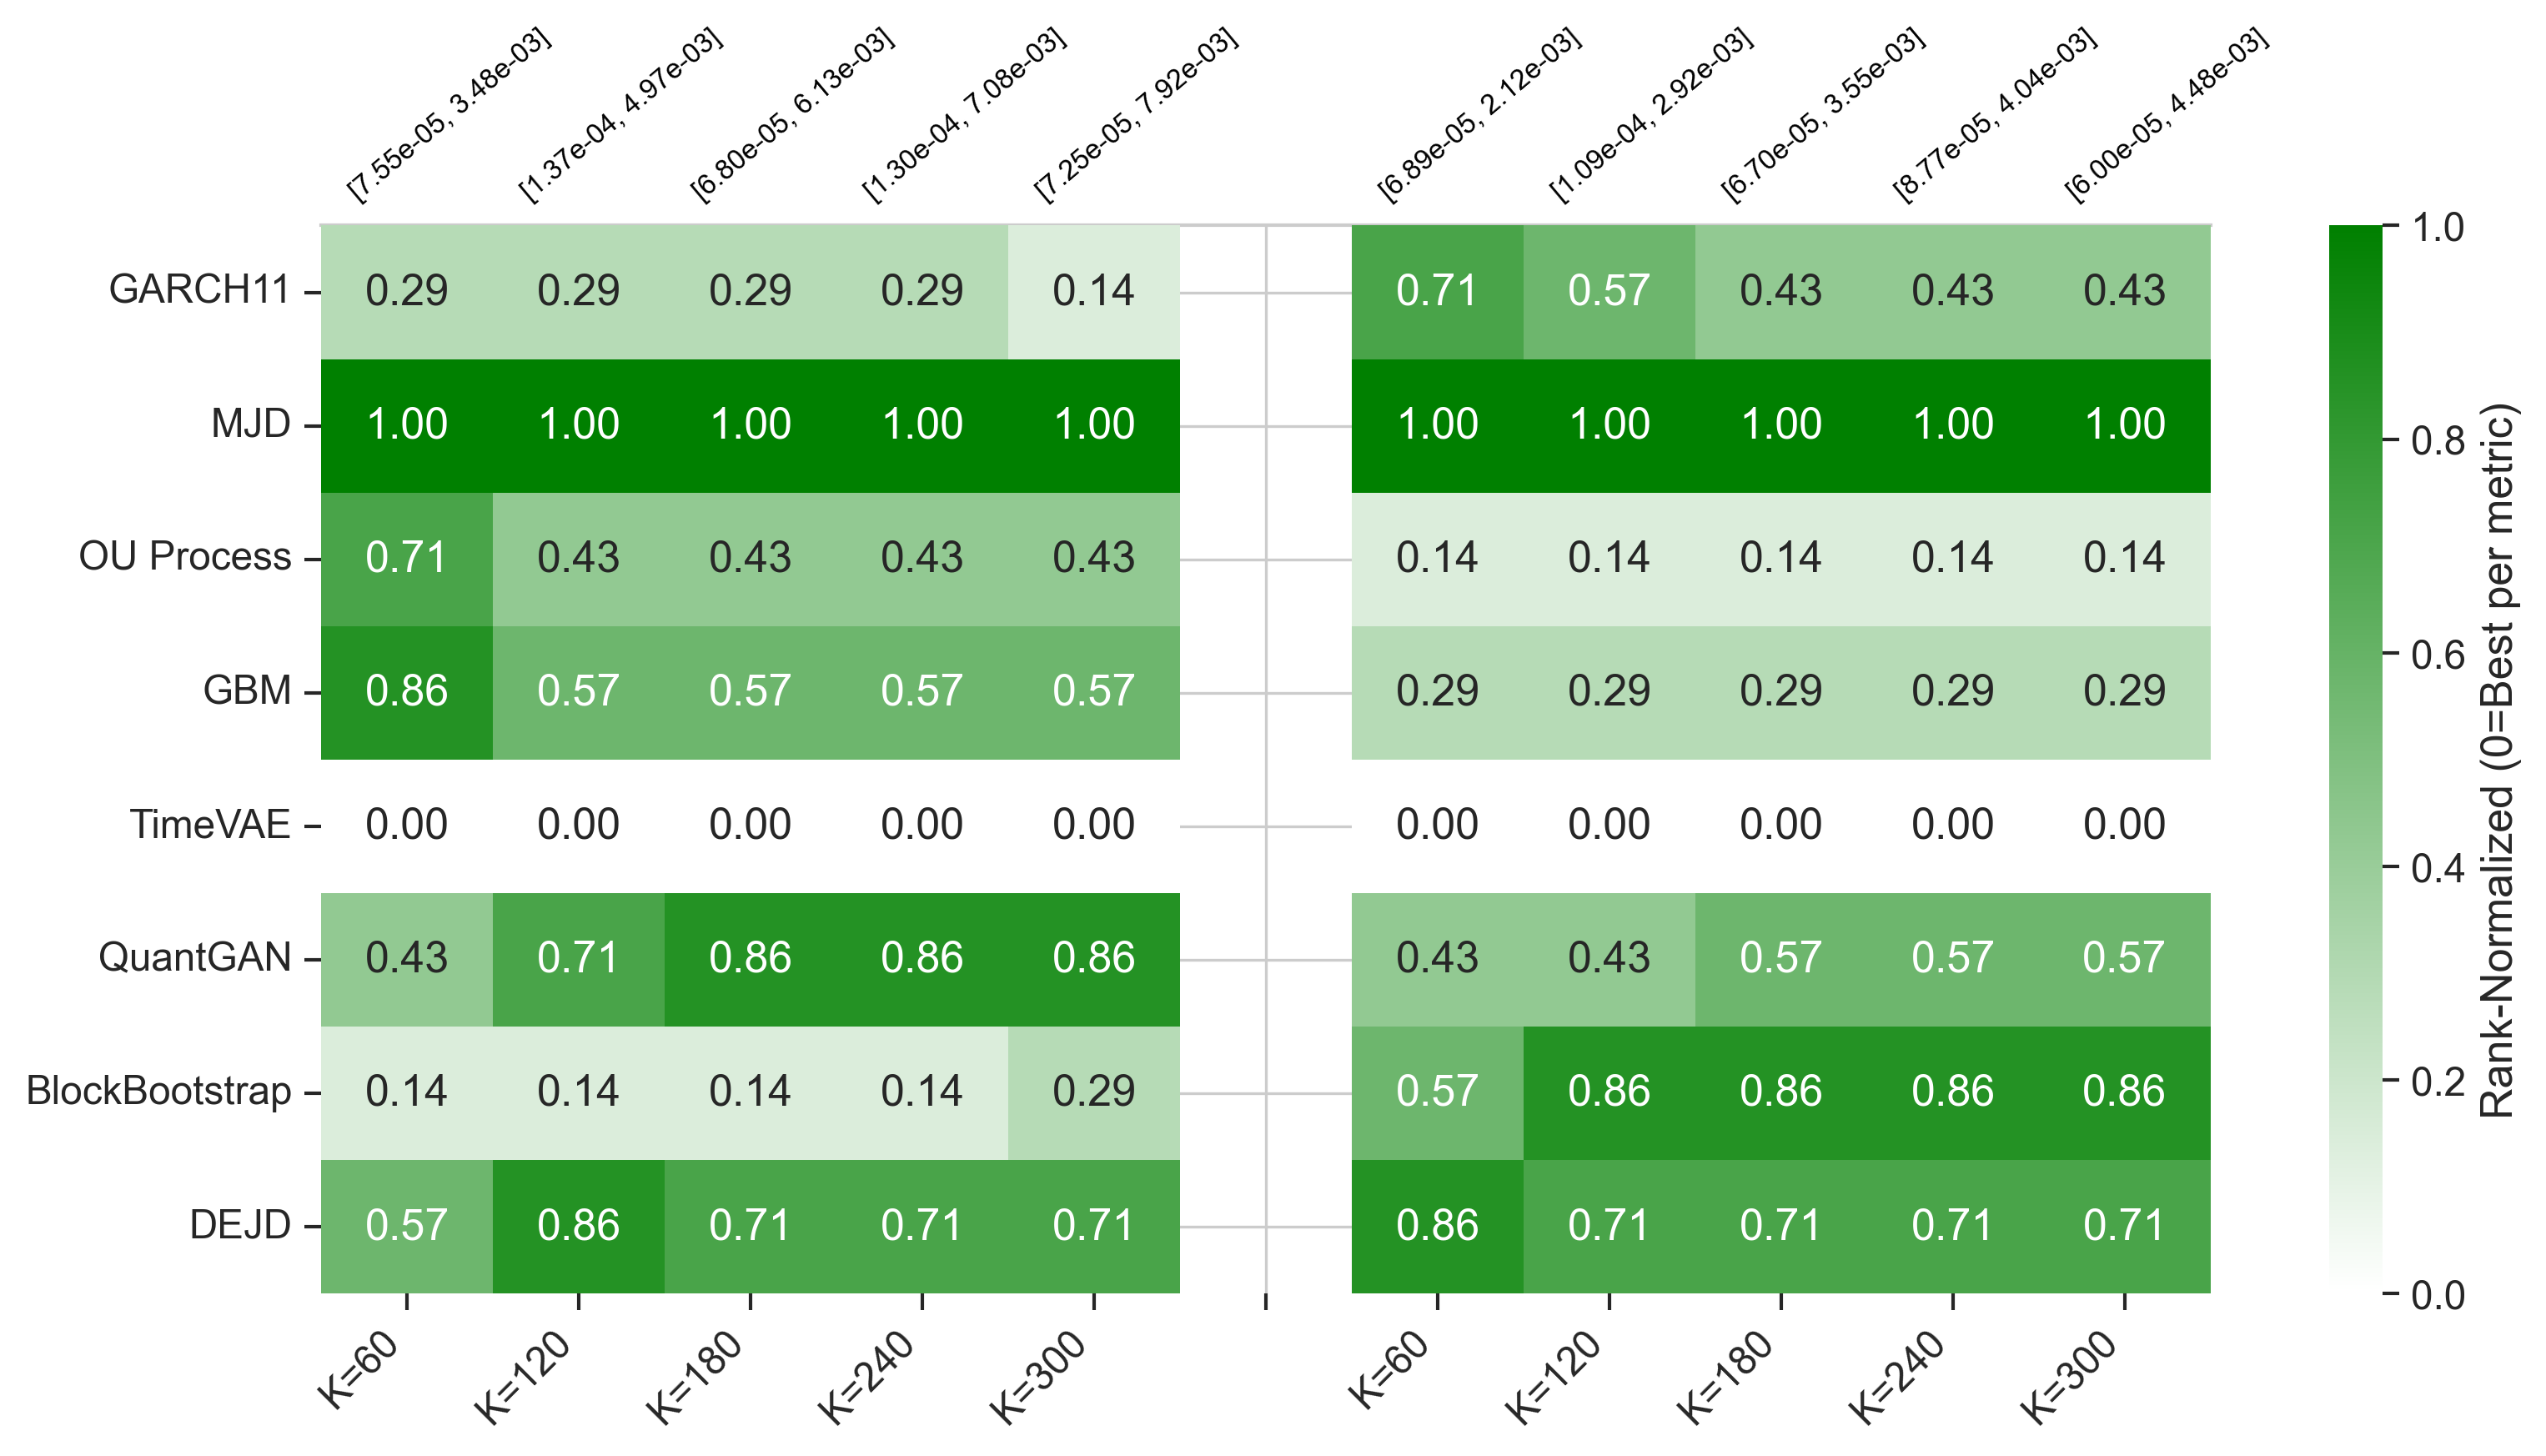
\includegraphics[width=0.9\textwidth,keepaspectratio]
  {../../results/ablation_studies/figure_3_metric_heatmaps_per_metric/figure_3_diversity_per_metric_ranknorm.png}
  \caption{Ablation study: diversity per-metric rank-normalized heatmap across sequence lengths.}
  \Description{Heatmap showing diversity metrics across sequence length ablations.}
  \label{fig:ablation_diversity}
\end{figure*}

\begin{figure*}[h]
  \centering
  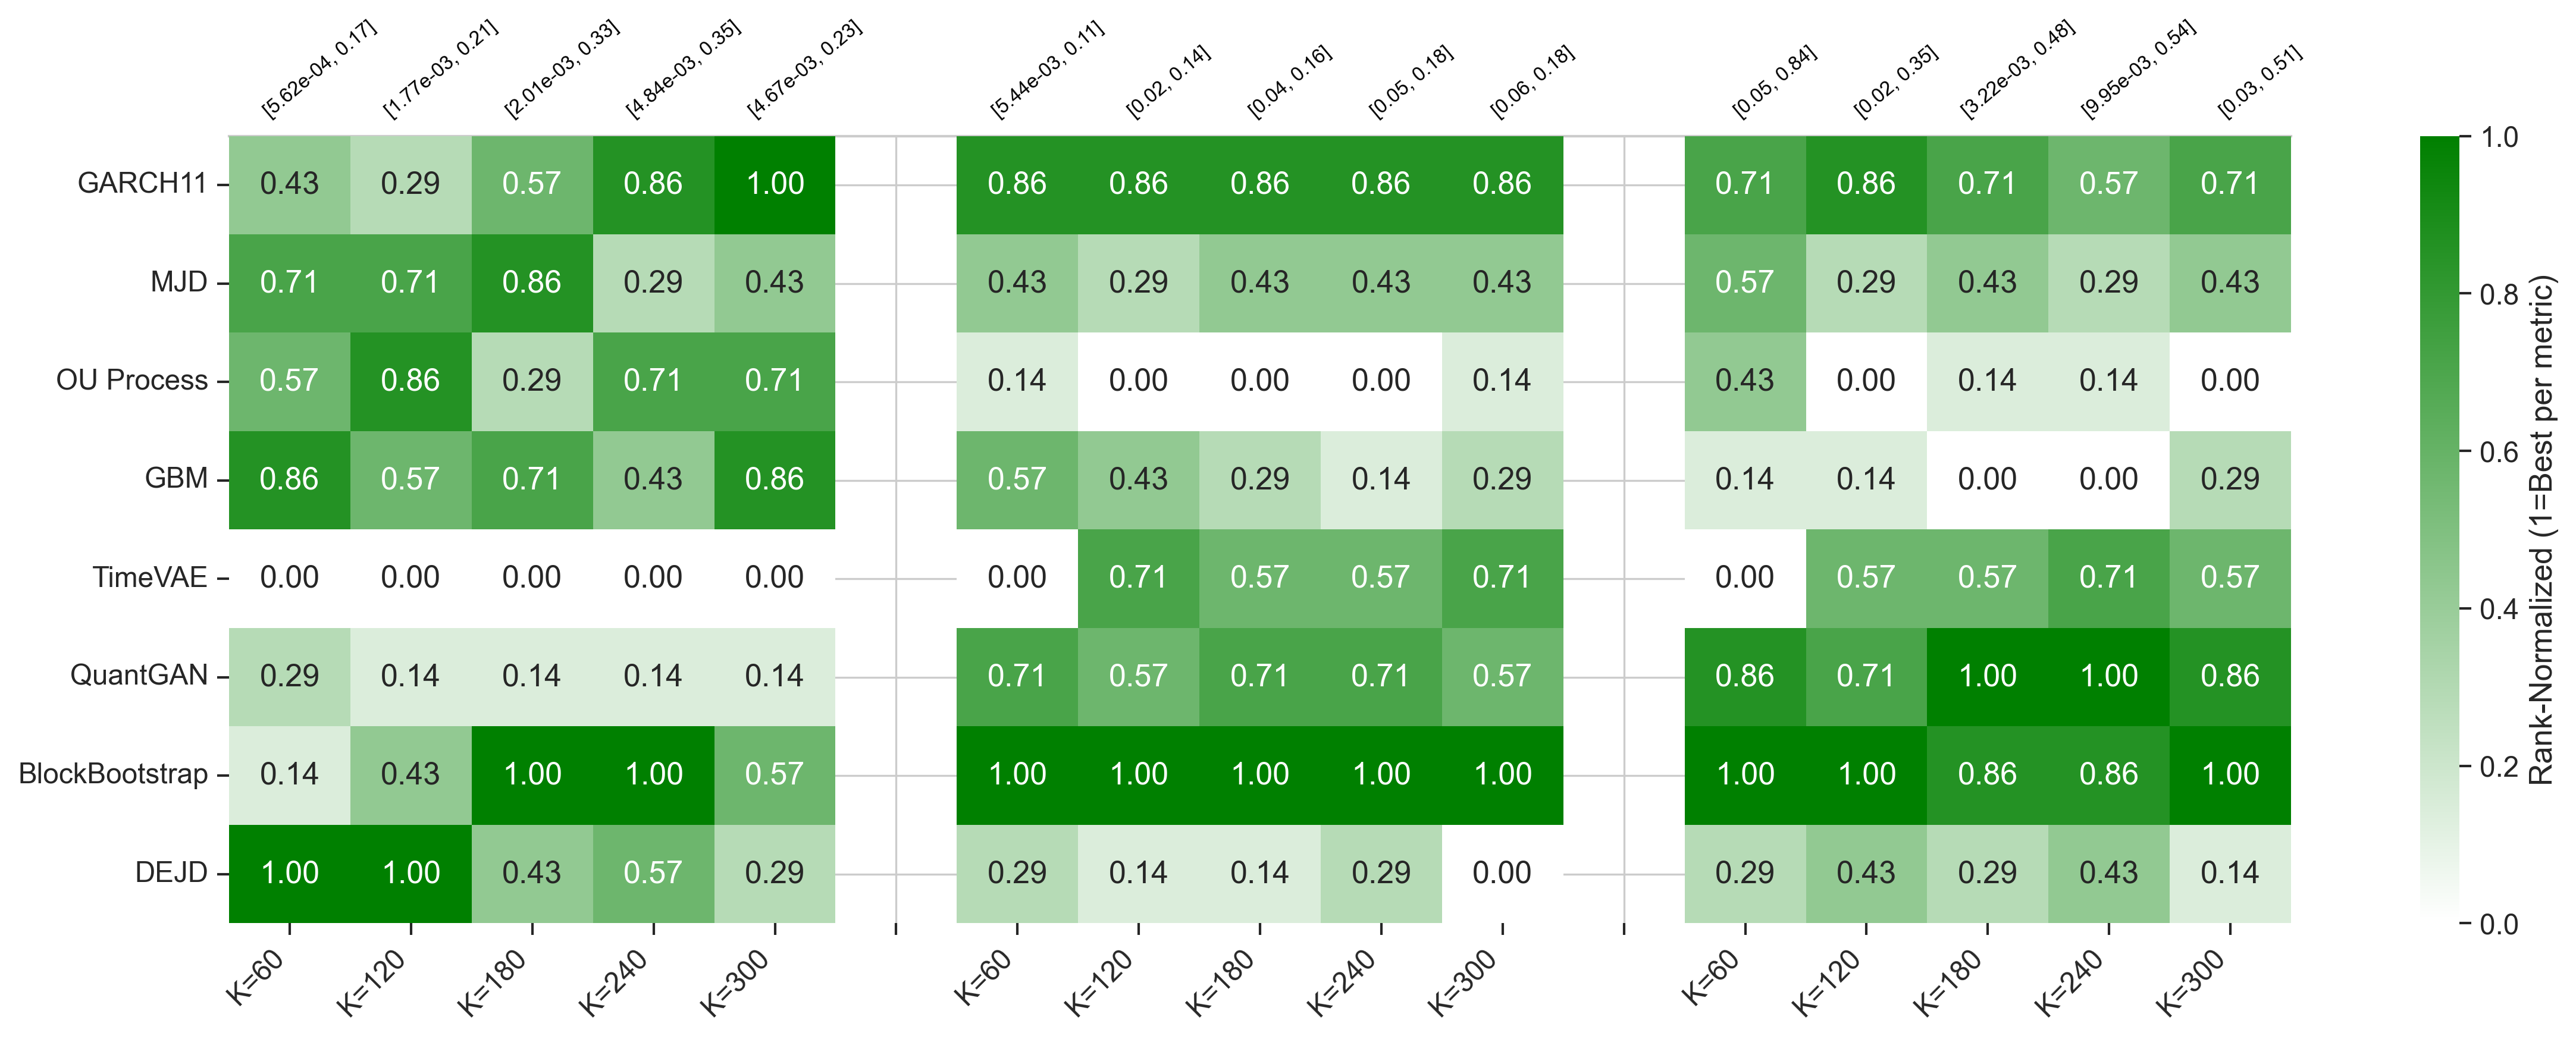
\includegraphics[width=0.9\textwidth,keepaspectratio]
  {../../results/ablation_studies/figure_3_metric_heatmaps_per_metric/figure_3_stylized-facts_per_metric_ranknorm.png}
  \caption{Ablation study: stylized-facts per-metric rank-normalized heatmap across sequence lengths.}
  \Description{Heatmap showing stylized-facts metrics across sequence length ablations.}
  \label{fig:ablation_stylized_facts}
\end{figure*}

\begin{figure*}[h]
  \centering
  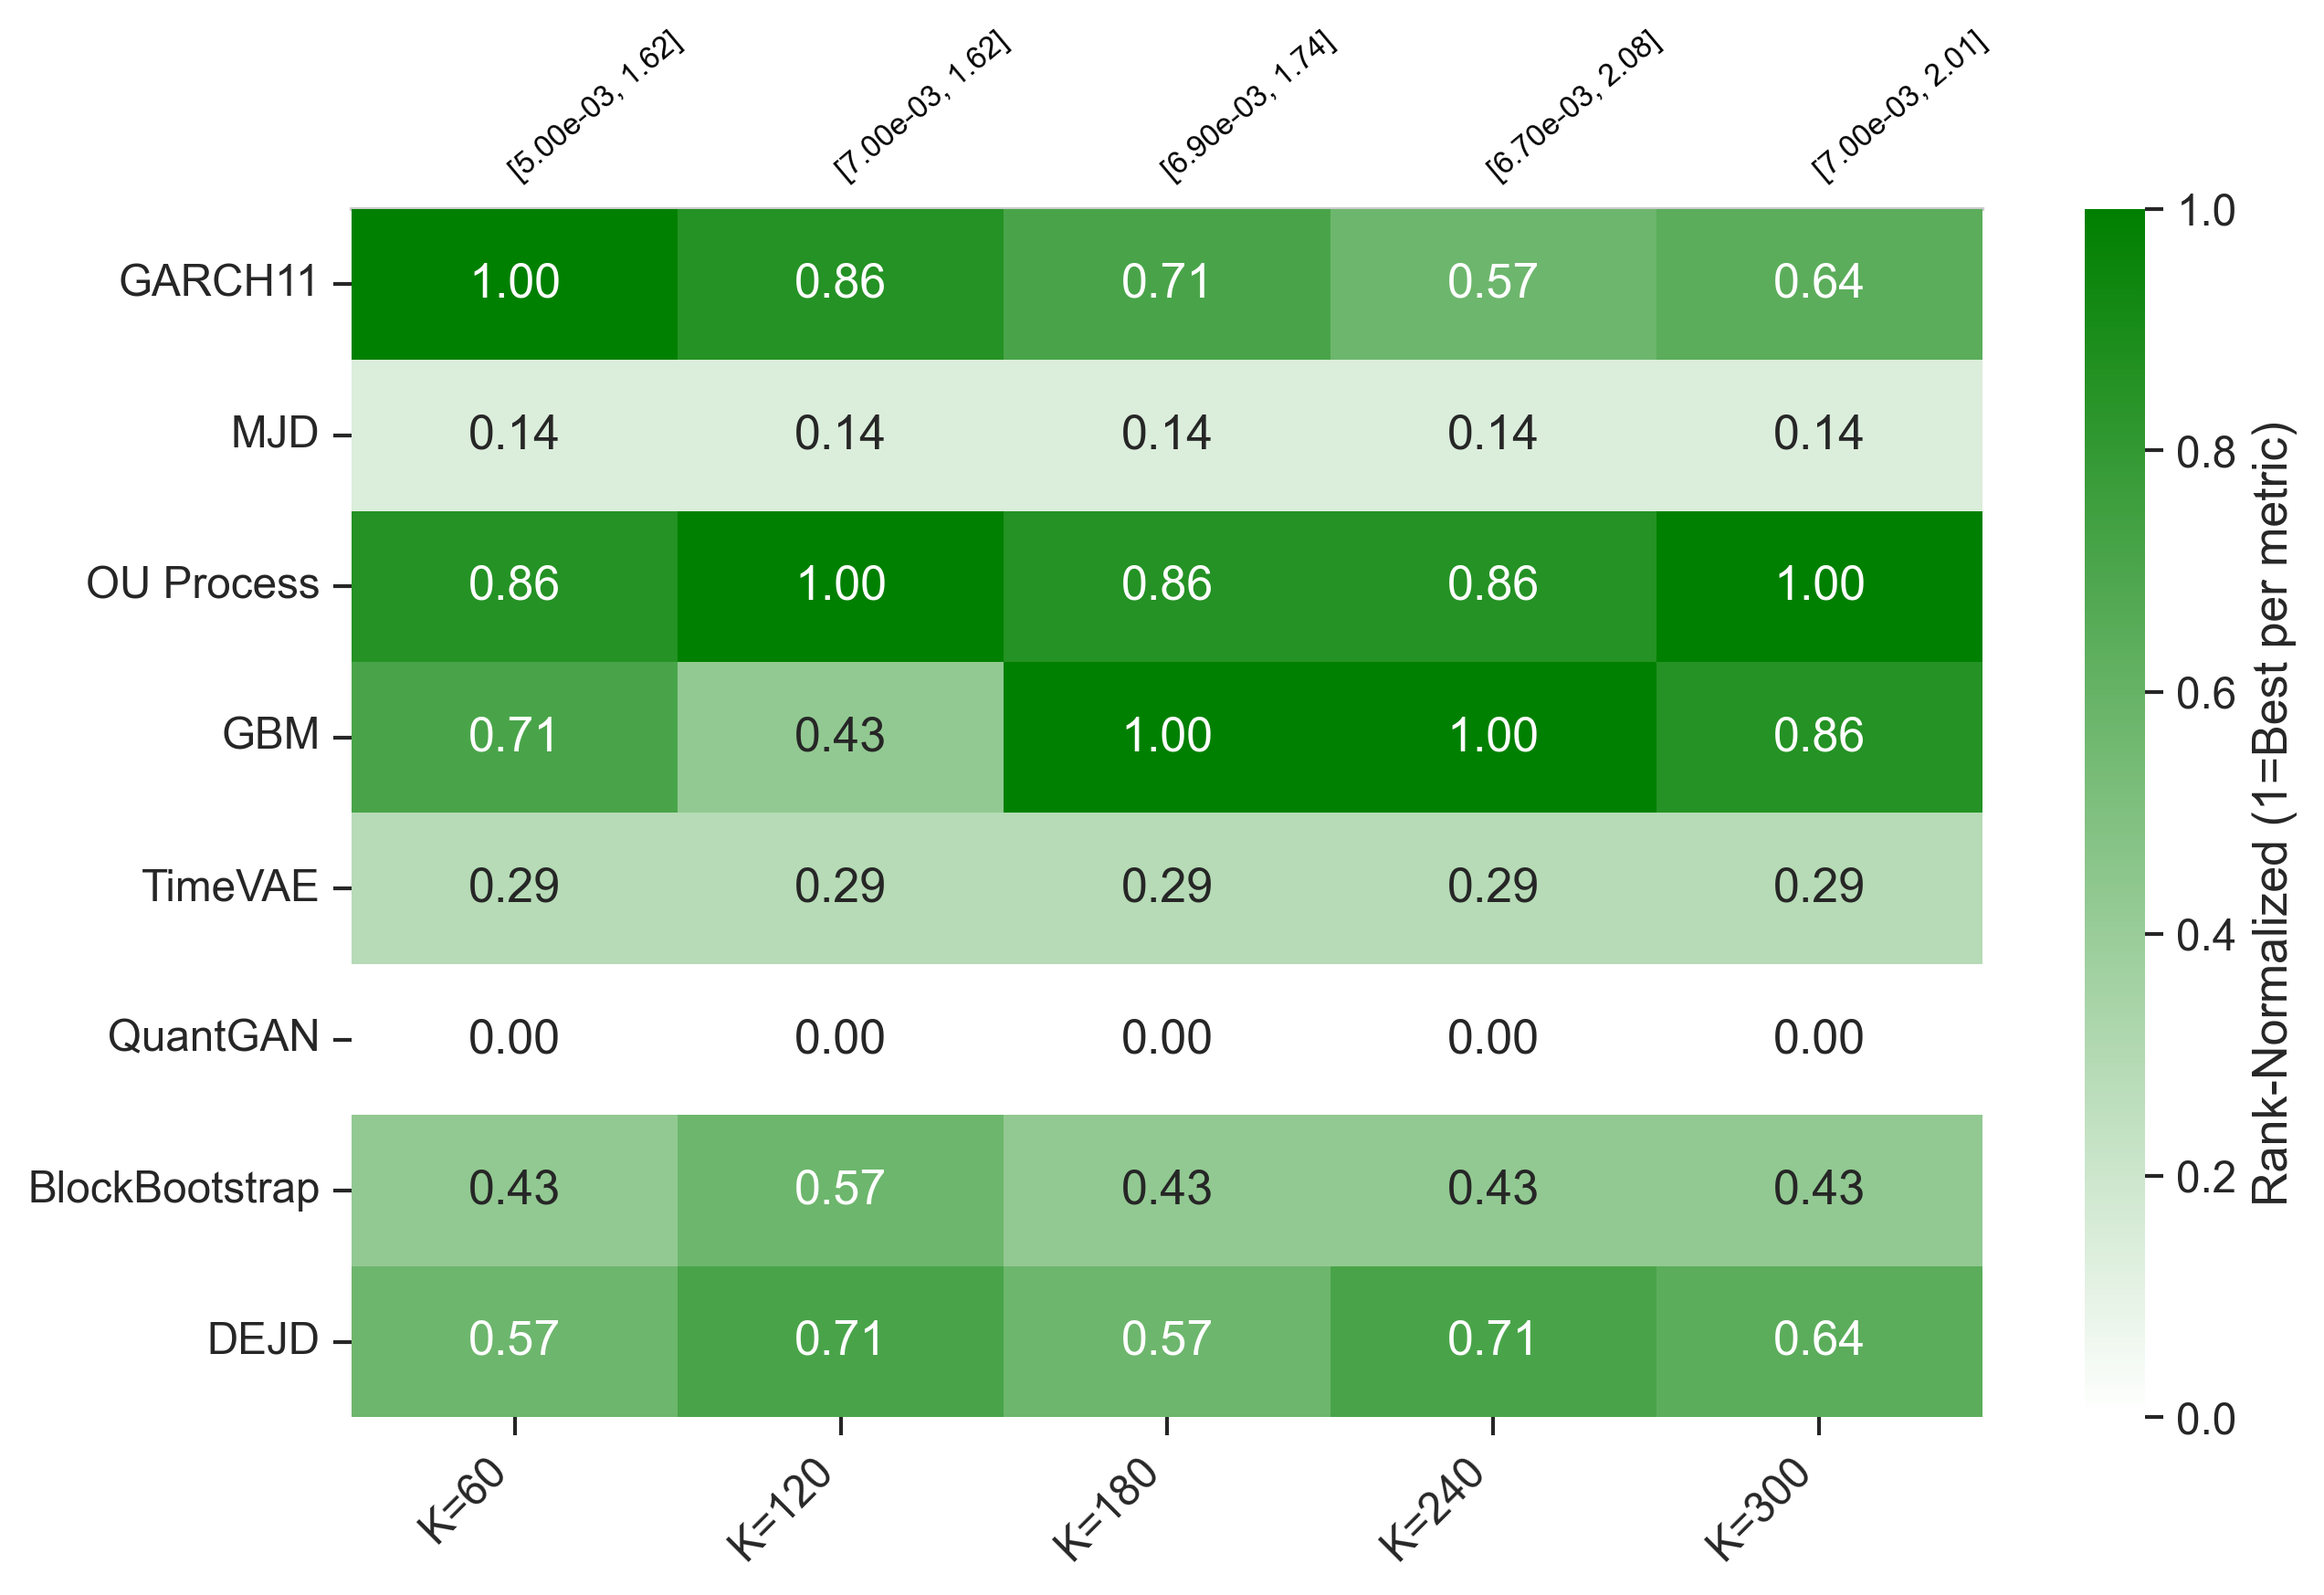
\includegraphics[width=0.9\textwidth,keepaspectratio]
  {../../results/ablation_studies/figure_3_metric_heatmaps_per_metric/figure_3_efficiency_per_metric_ranknorm.png}
  \caption{Ablation study: efficiency per-metric rank-normalized heatmap across sequence lengths.}
  \Description{Heatmap showing efficiency metrics across sequence length ablations.}
  \label{fig:ablation_efficiency}
\end{figure*}

\begin{figure*}[h]
  \centering
  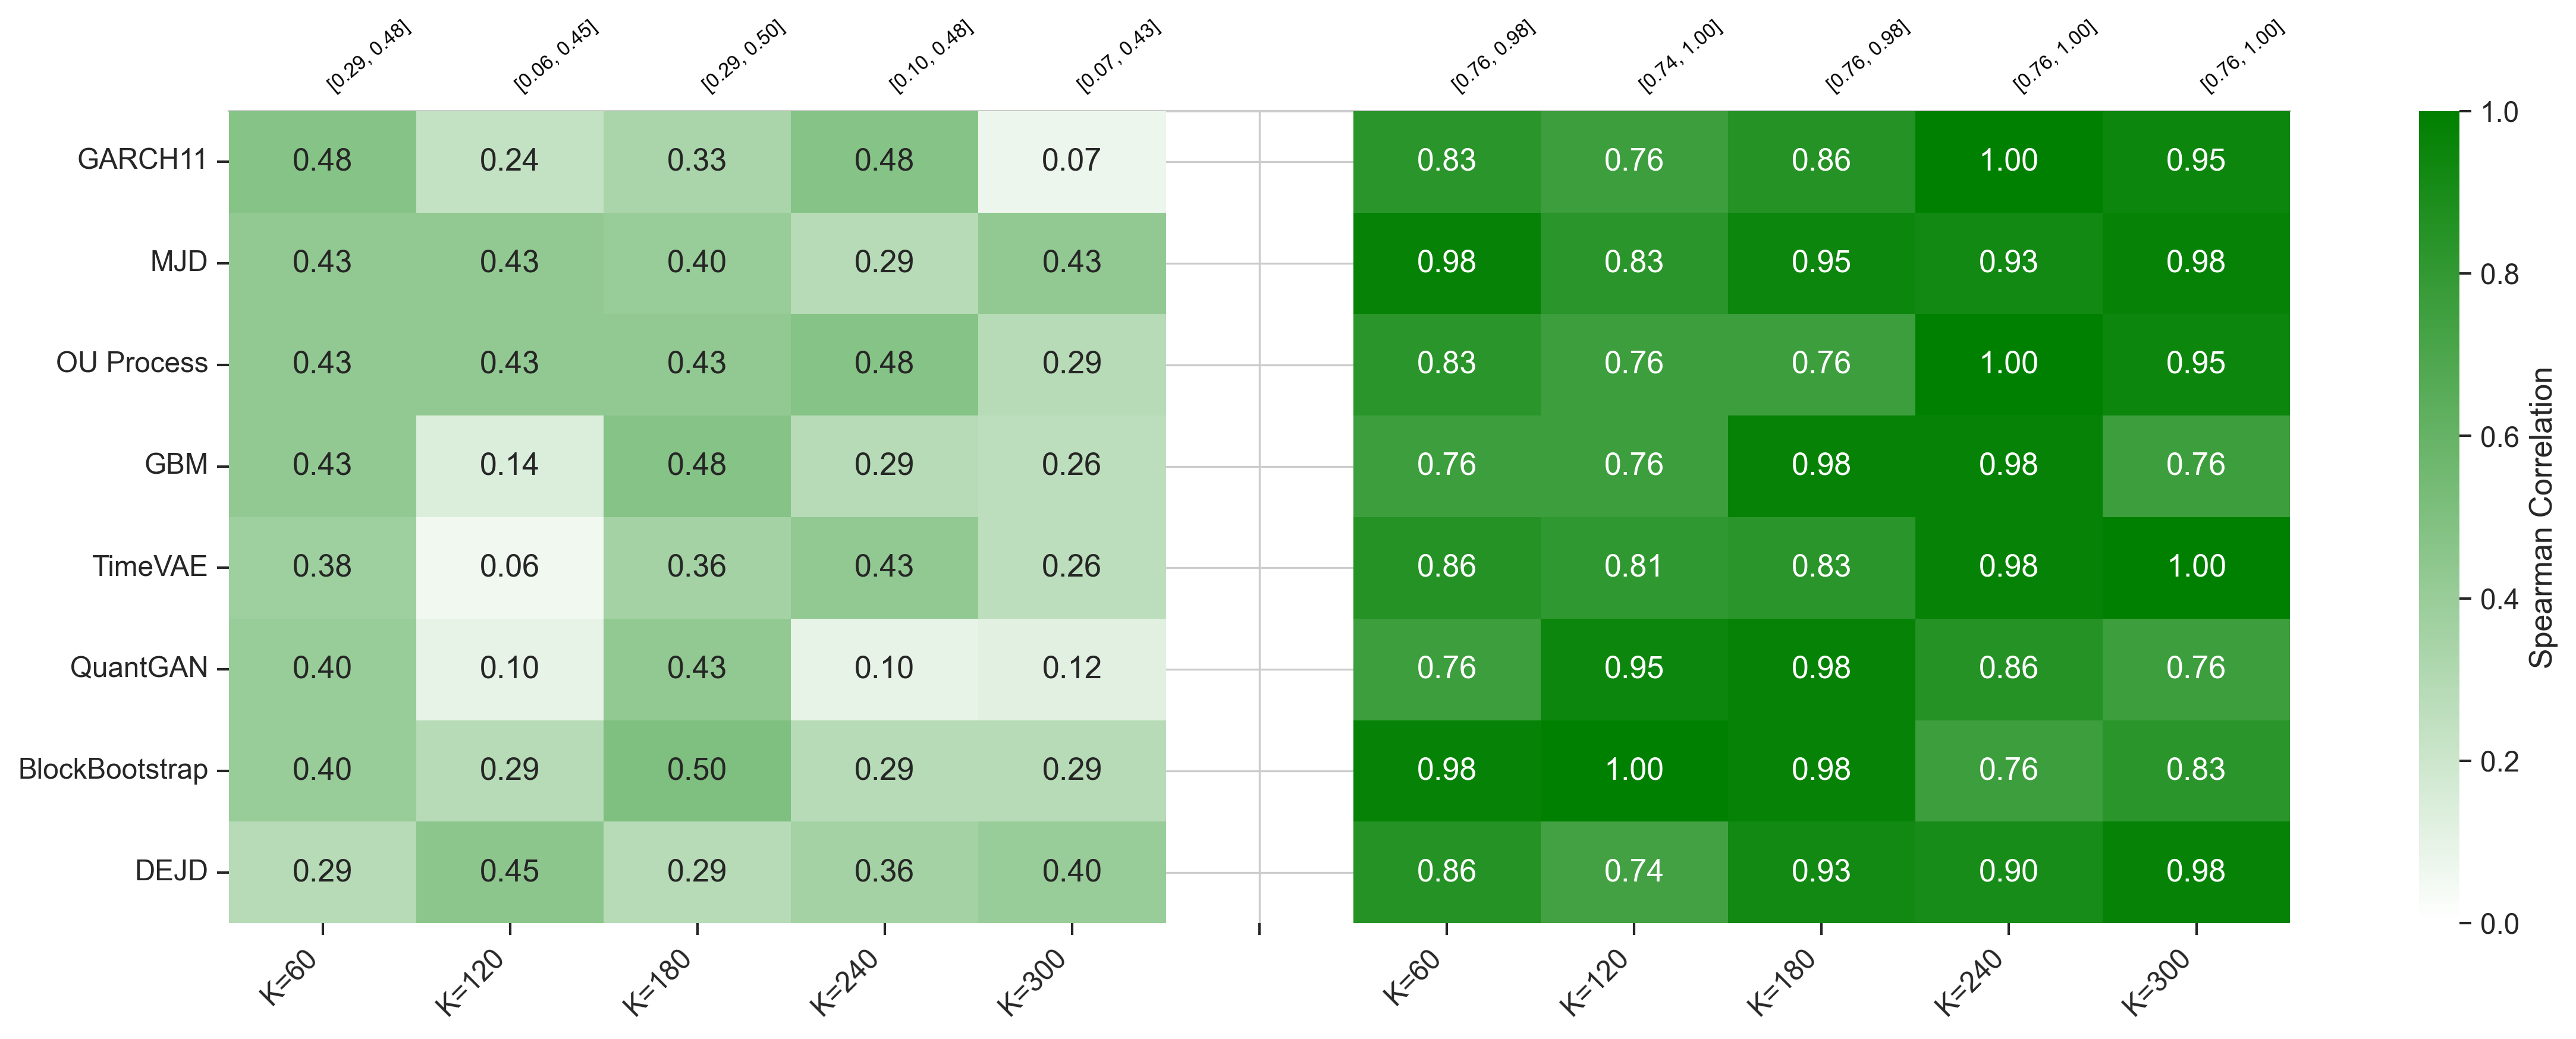
\includegraphics[width=0.9\textwidth,keepaspectratio]
  {../../results/ablation_studies/figure_3_metric_heatmaps_per_metric/figure_3_utility_spearman_and_mixed_per_seq.png}
  \caption{Ablation study: utility (Spearman) per-sequence-length comparison across hedger algorithms between real and sythetic data.}
  \Description{Heatmap or plot showing utility Spearman correlations per sequence length.}
  \label{fig:ablation_utility_spearman}
\end{figure*}

      \begin{figure*}[h]
      \centering
      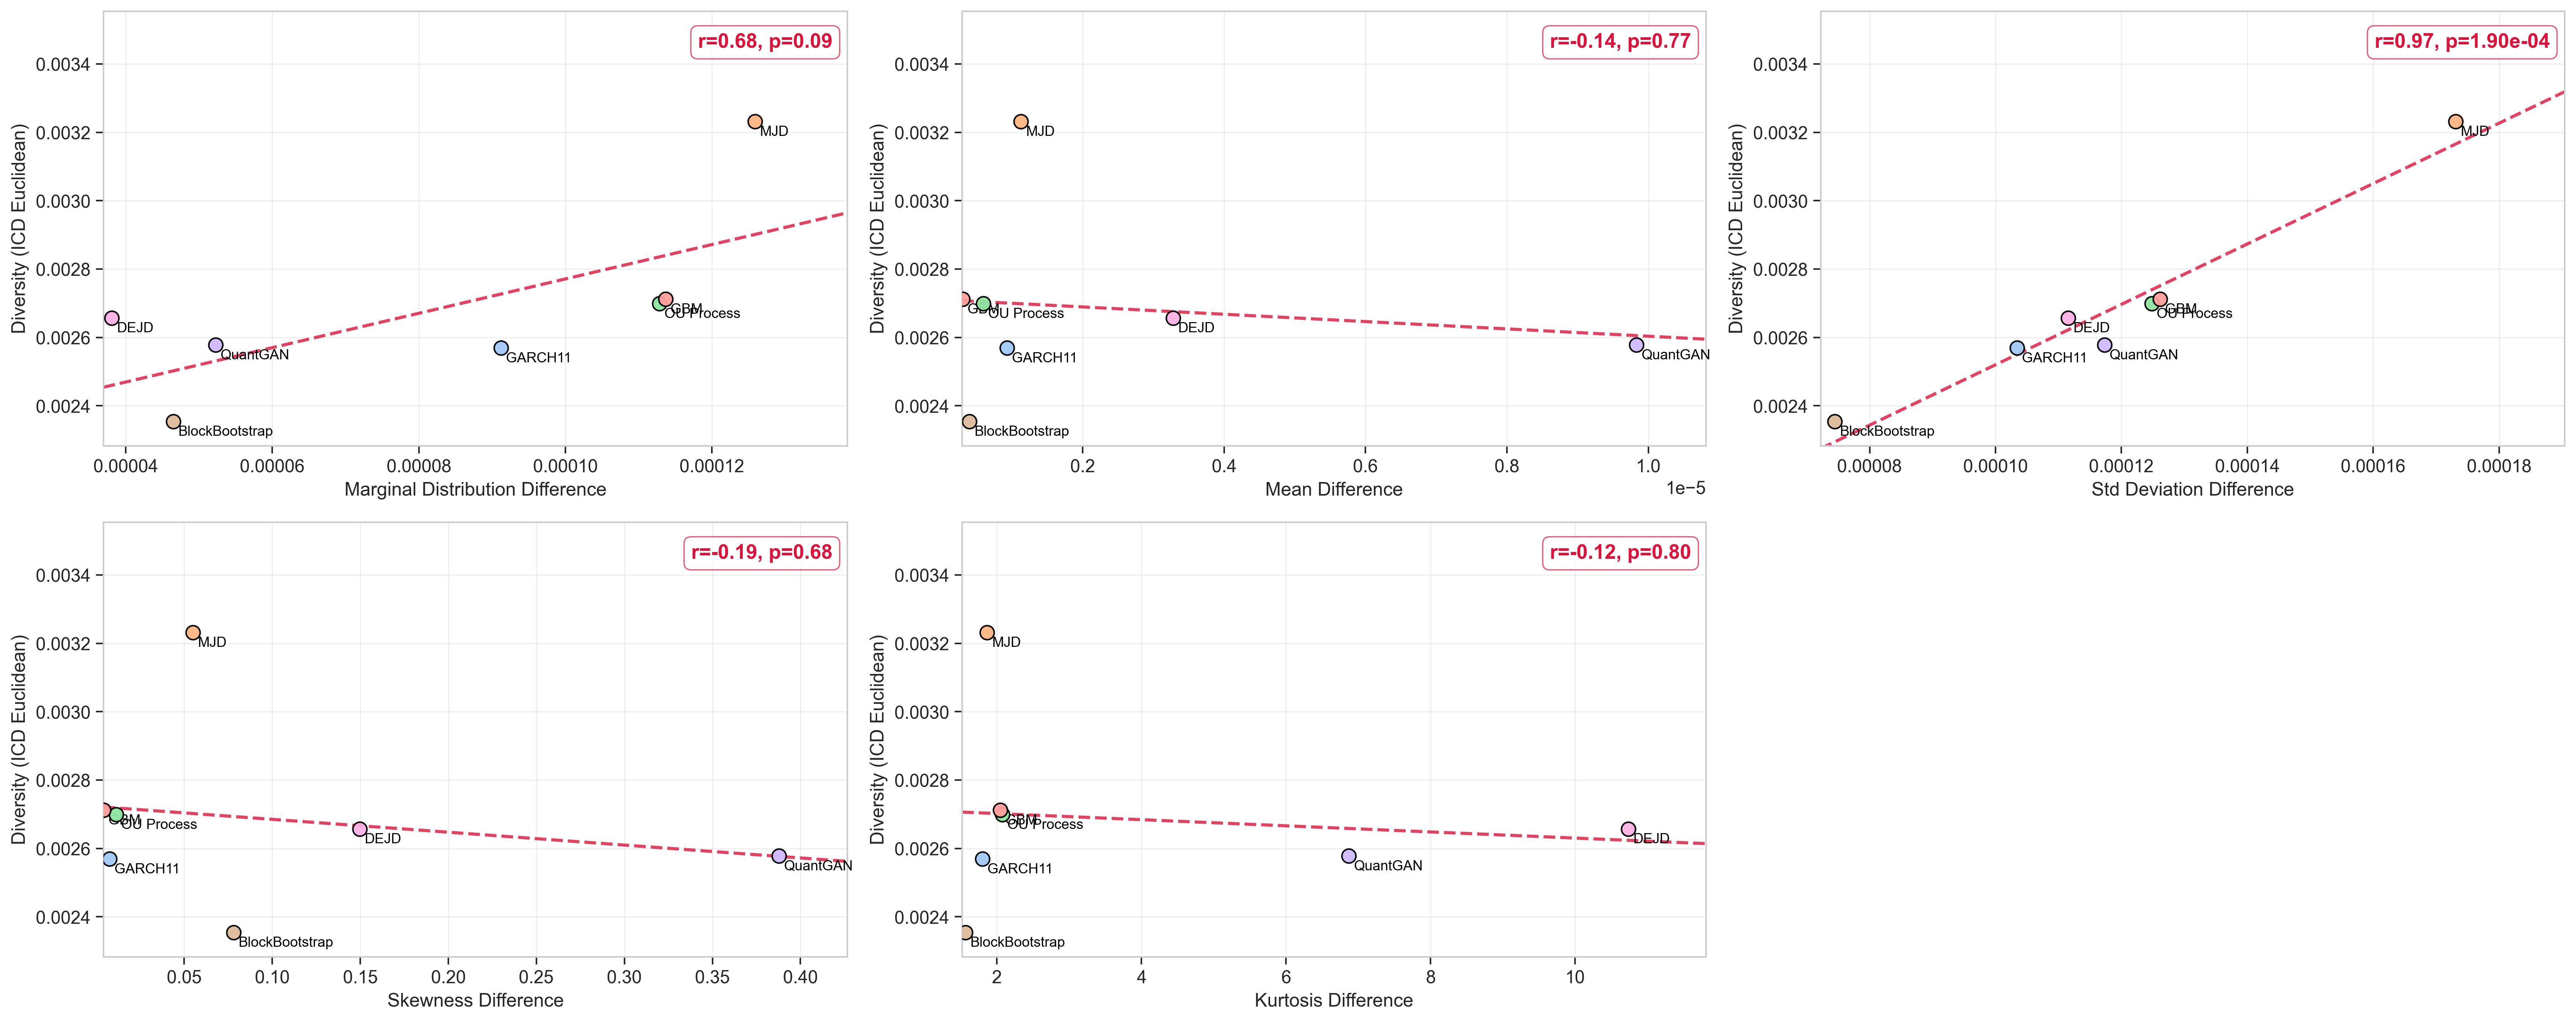
\includegraphics[width=\textwidth,height=10cm,keepaspectratio]
      {../../results/appendix/figure_5_fidelity_vs_diversity/figure_5_icd_euclidean_2x3_grid.png}
      \caption{Scatter plots and linear regression analysis showing the relationship between 
      fidelity metrics (MDD, MD, SDD, SD, KD, by row) and intra-class Euclidean distance (ICD-ED) 
      across all SDGFTS models. Each subplot displays the fitted regression line with 
      corresponding R² value and p-value, indicating the strength and statistical significance 
      of the linear relationship between fidelity and diversity.}
      \Description{A heatmap displaying the normalized rankings of diversity metrics for
      different SDGFTS models, highlighting the performance scores and their implications for model diversity.}
      \label{fig:eclidian_fidelity_diversity}
    \end{figure*}

      \begin{figure*}[h]
      \centering
      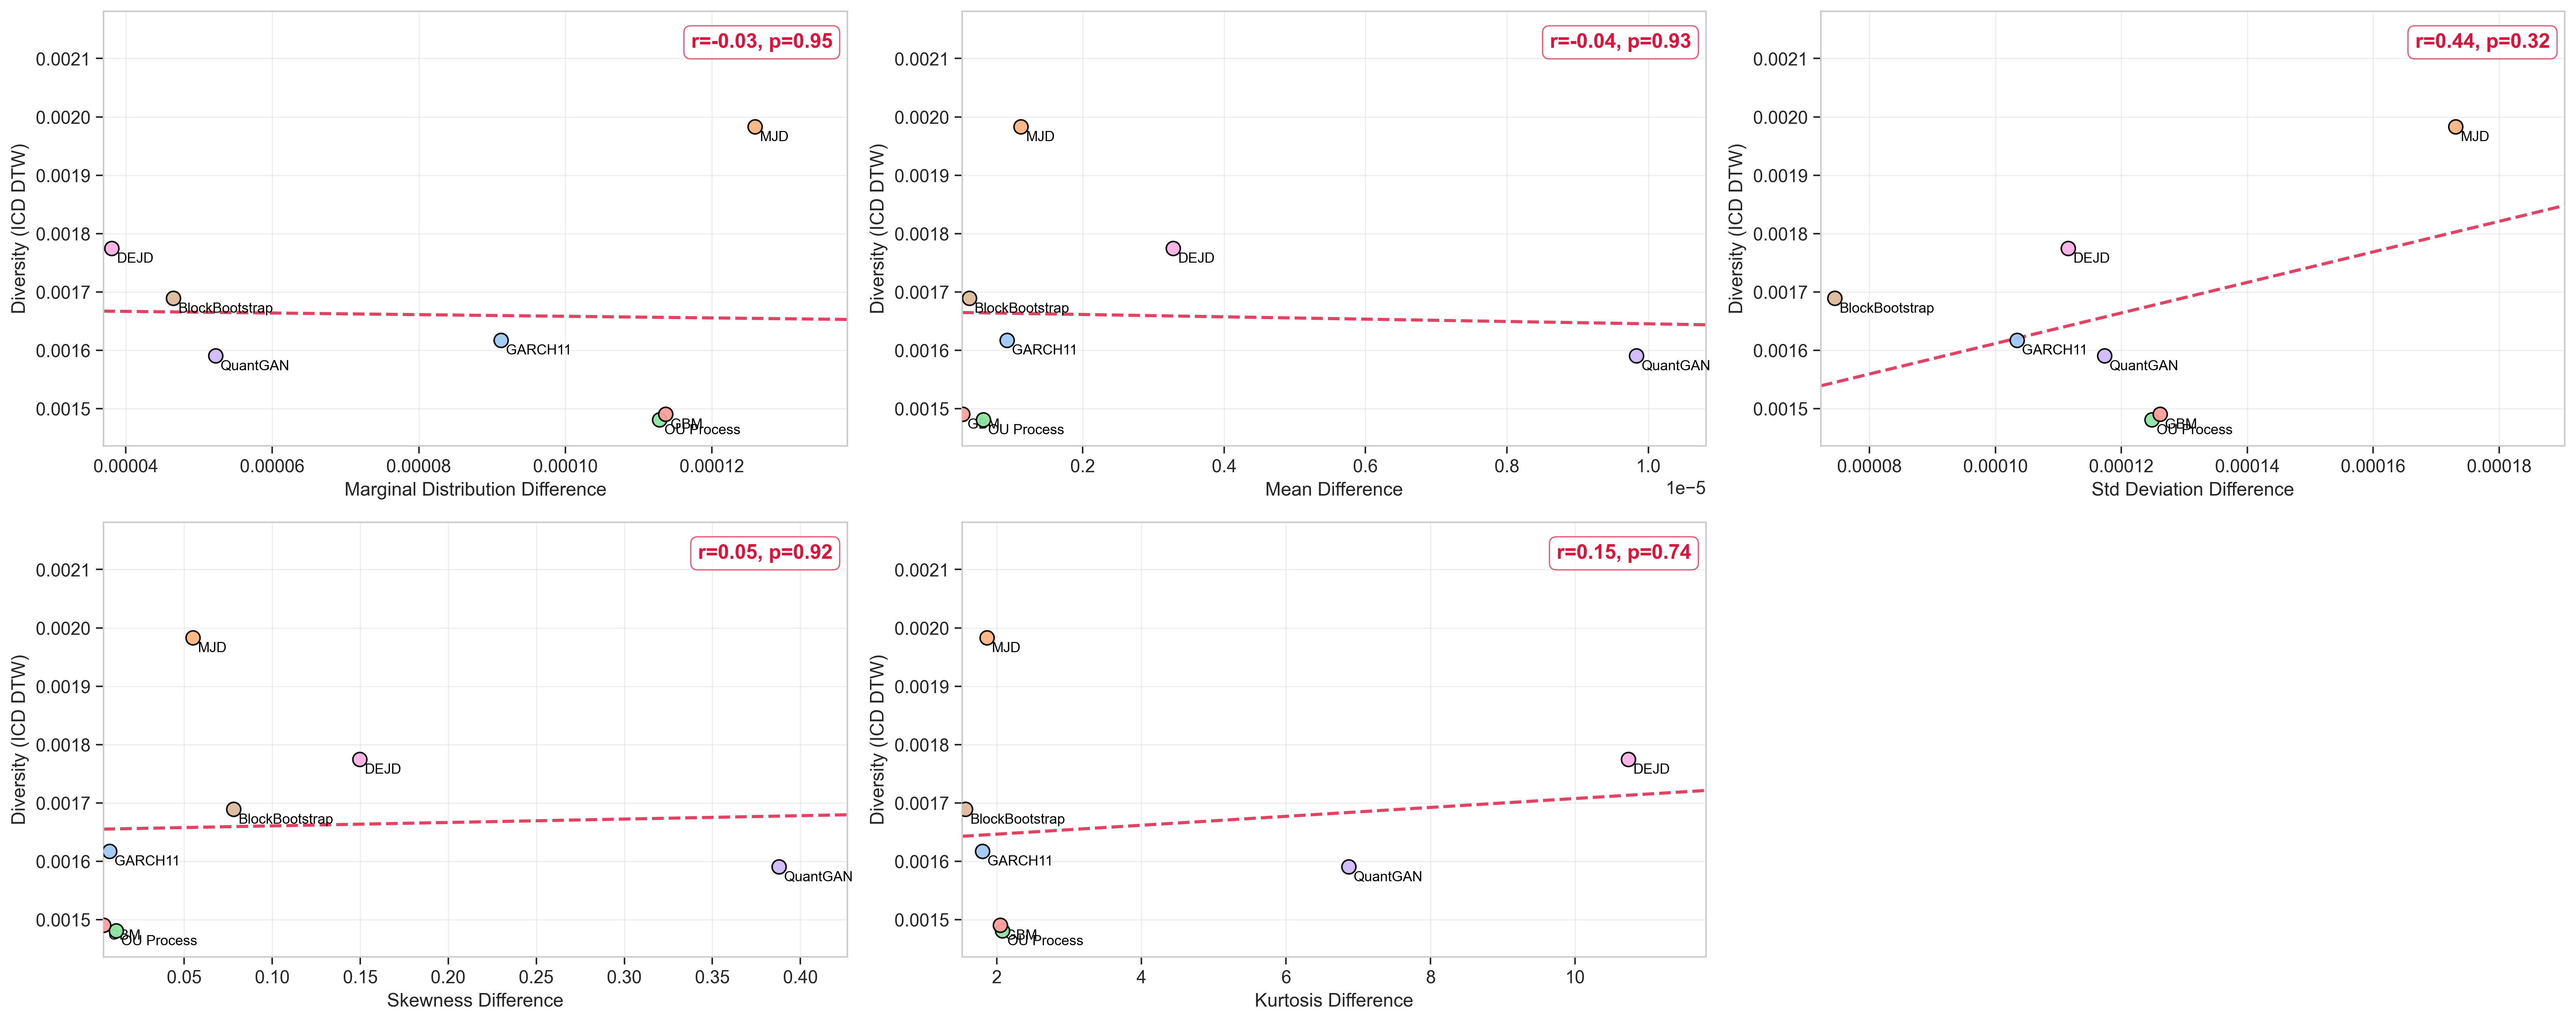
\includegraphics[width=\textwidth,height=10cm,keepaspectratio]
      {../../results/appendix/figure_5_fidelity_vs_diversity/figure_5_icd_dtw_2x3_grid.png}
      \caption{Scatter plots and linear regression analysis showing the relationship between 
      fidelity metrics (MDD, MD, SDD, SD, KD, by row) and intra-class DTW distance (ICD-DTW) 
      across all SDGFTS models. Each subplot displays the fitted regression line with 
      corresponding R² value and p-value, indicating the strength and statistical significance 
      of the linear relationship between fidelity and diversity measured by DTW.}
      \Description{Scatter plots showing the correlation between fidelity metrics and 
      ICD-DTW diversity across different SDGFTS models.}
      \label{fig:dtw_fidelity_diversity}
    \end{figure*}

      \begin{figure*}[h]
      \centering
      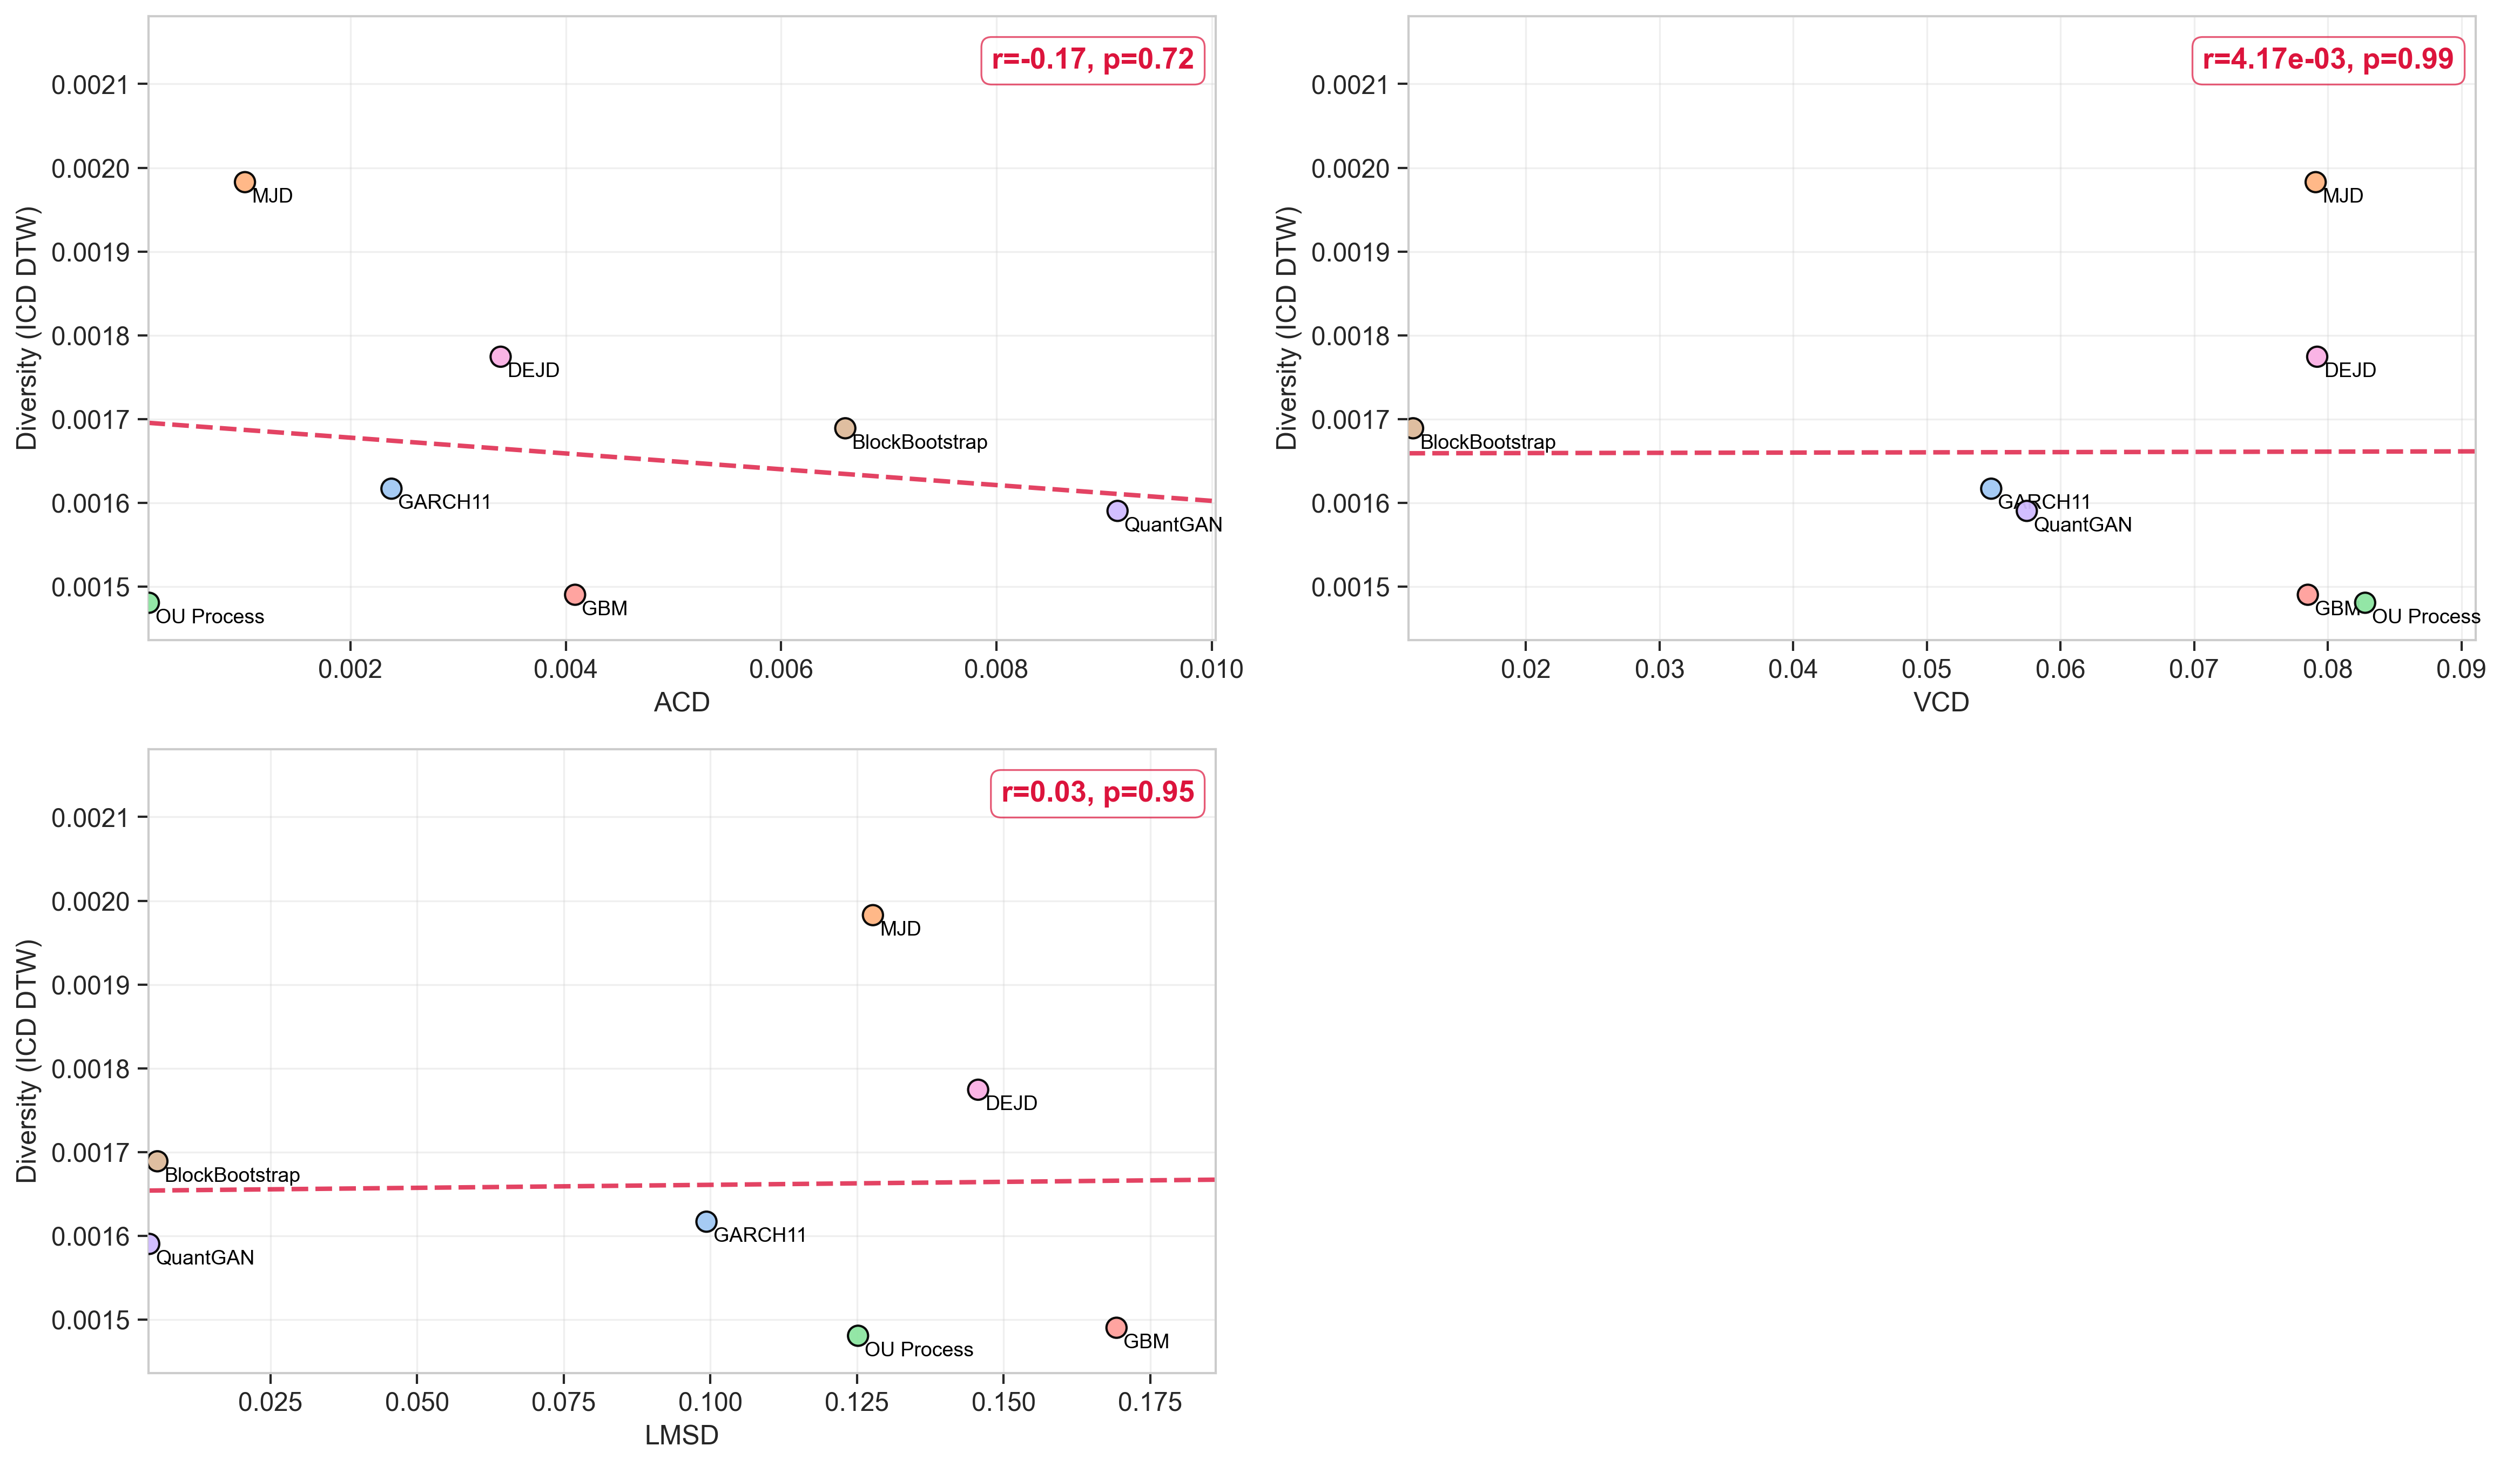
\includegraphics[width=\textwidth,height=10cm,keepaspectratio]
      {../../results/appendix/figure_6_stylized_facts_vs_diversity/figure_6_icd_dtw_2x2_grid.png}
      \caption{Scatter plots showing the relationship between stylized facts metrics 
      (ACD, volatility clustering, and LMSD) and intra-class DTW distance (ICD-DTW) 
      across all SDGFTS models. Each point represents a model, with trend lines 
      indicating correlation direction and strength.}
      \Description{Scatter plots illustrating the correlation between stylized facts 
      metrics and ICD-DTW diversity across different models.}
      \label{fig:dtw_stylized_facts_diversity}
    \end{figure*}

\section{Supplementary t-SNE Visualizations}

\begin{figure*}[h]
  \centering
  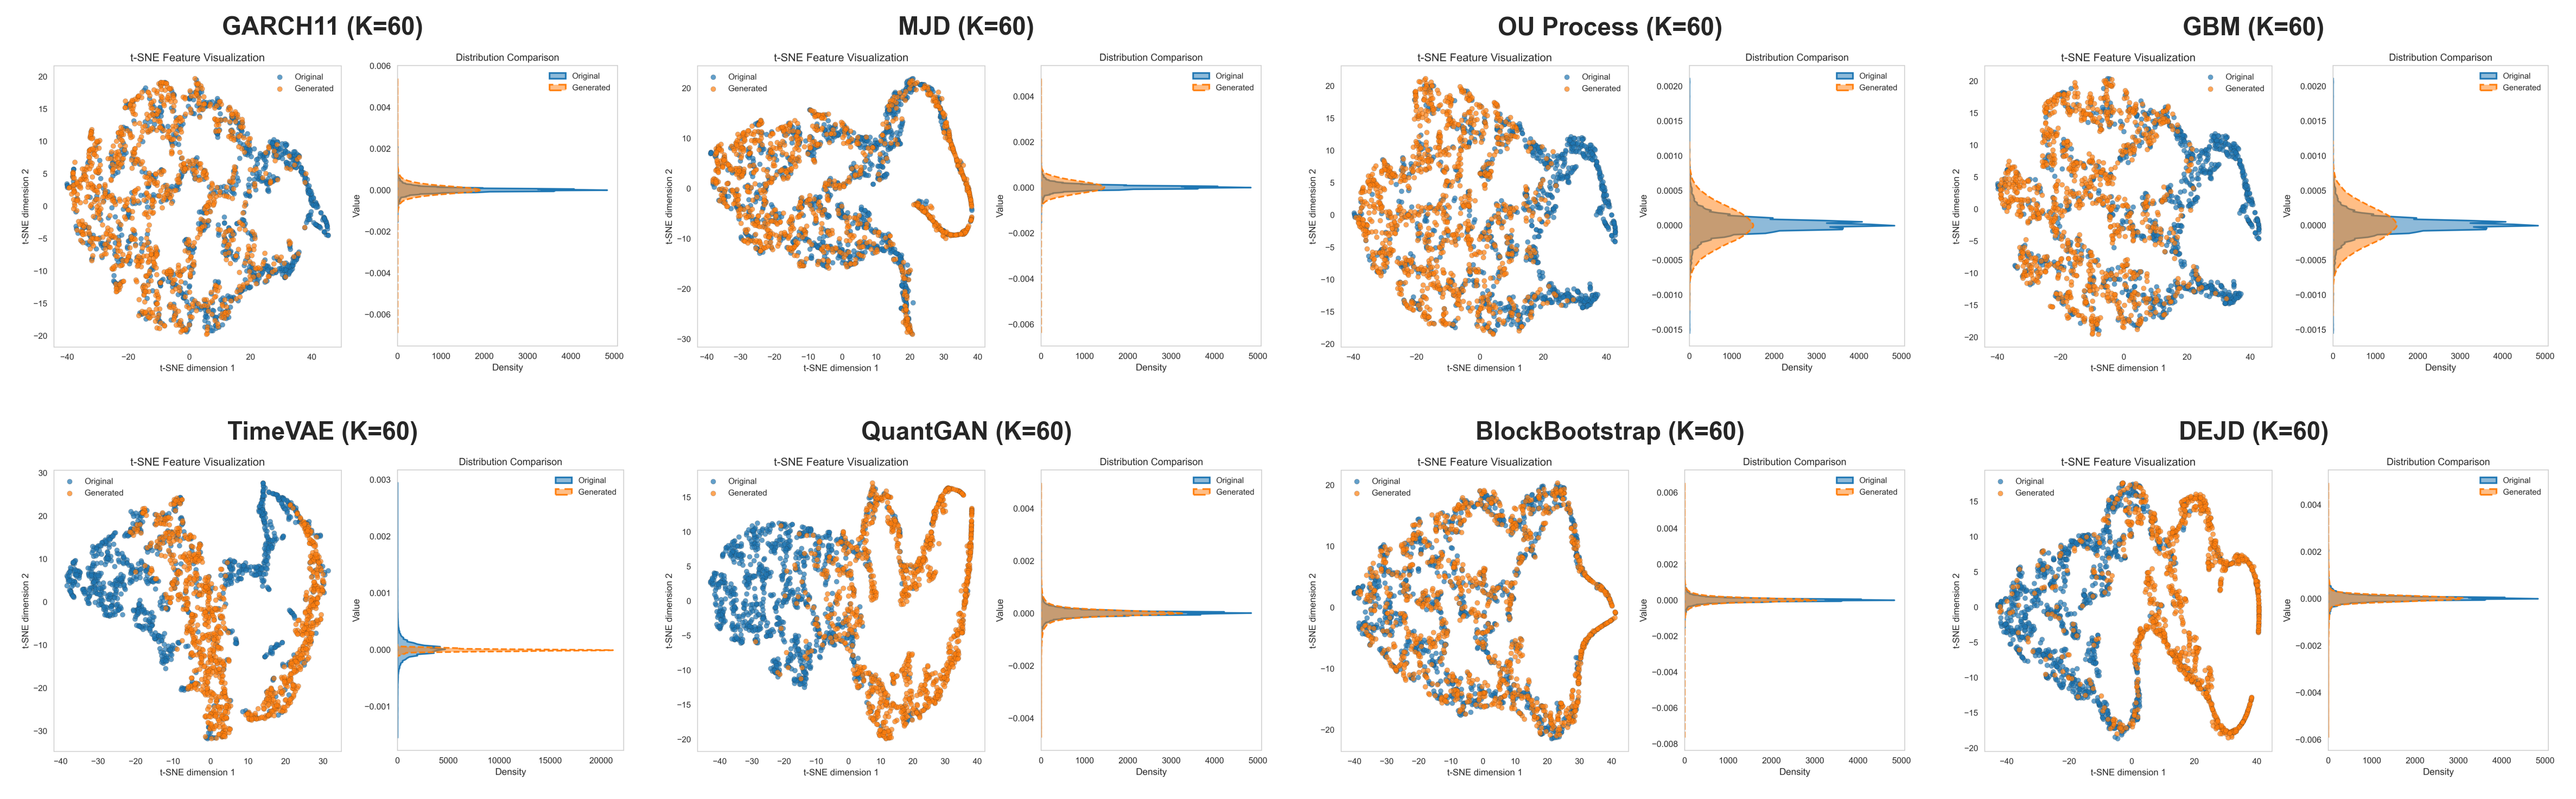
\includegraphics[width=0.9\textwidth,keepaspectratio]
  {../../results/appendix/figure_4_tsne_supplementary/figure_4_seq_60.png}
  \caption{Supplementary t-SNE visualization for sequence length 60 minutes.}
  \Description{t-SNE embeddings comparing real and synthetic data for 60-minute sequences.}
  \label{fig:tsne_seq_60}
\end{figure*}

\begin{figure*}[h]
  \centering
  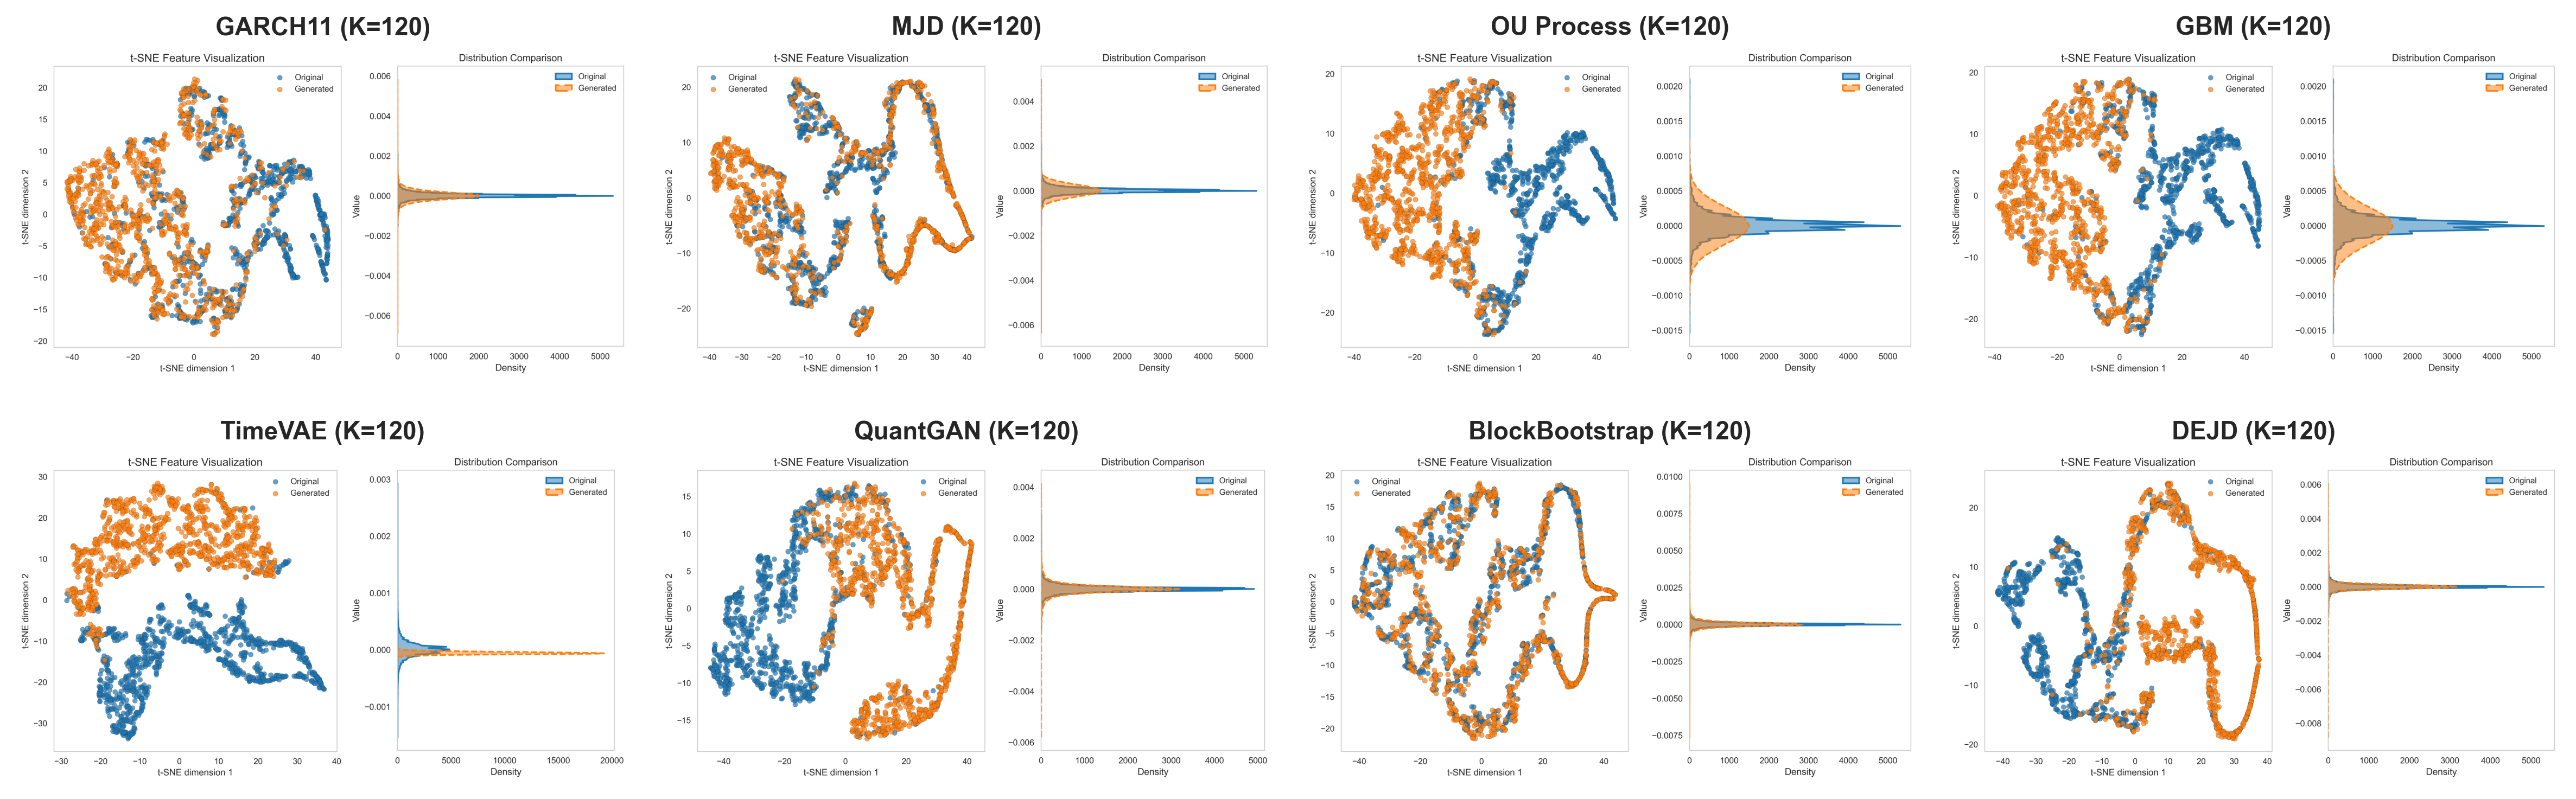
\includegraphics[width=0.9\textwidth,keepaspectratio]
  {../../results/appendix/figure_4_tsne_supplementary/figure_4_seq_120.png}
  \caption{Supplementary t-SNE visualization for sequence length 120 minutes.}
  \Description{t-SNE embeddings comparing real and synthetic data for 120-minute sequences.}
  \label{fig:tsne_seq_120}
\end{figure*}

\begin{figure*}[h]
  \centering
  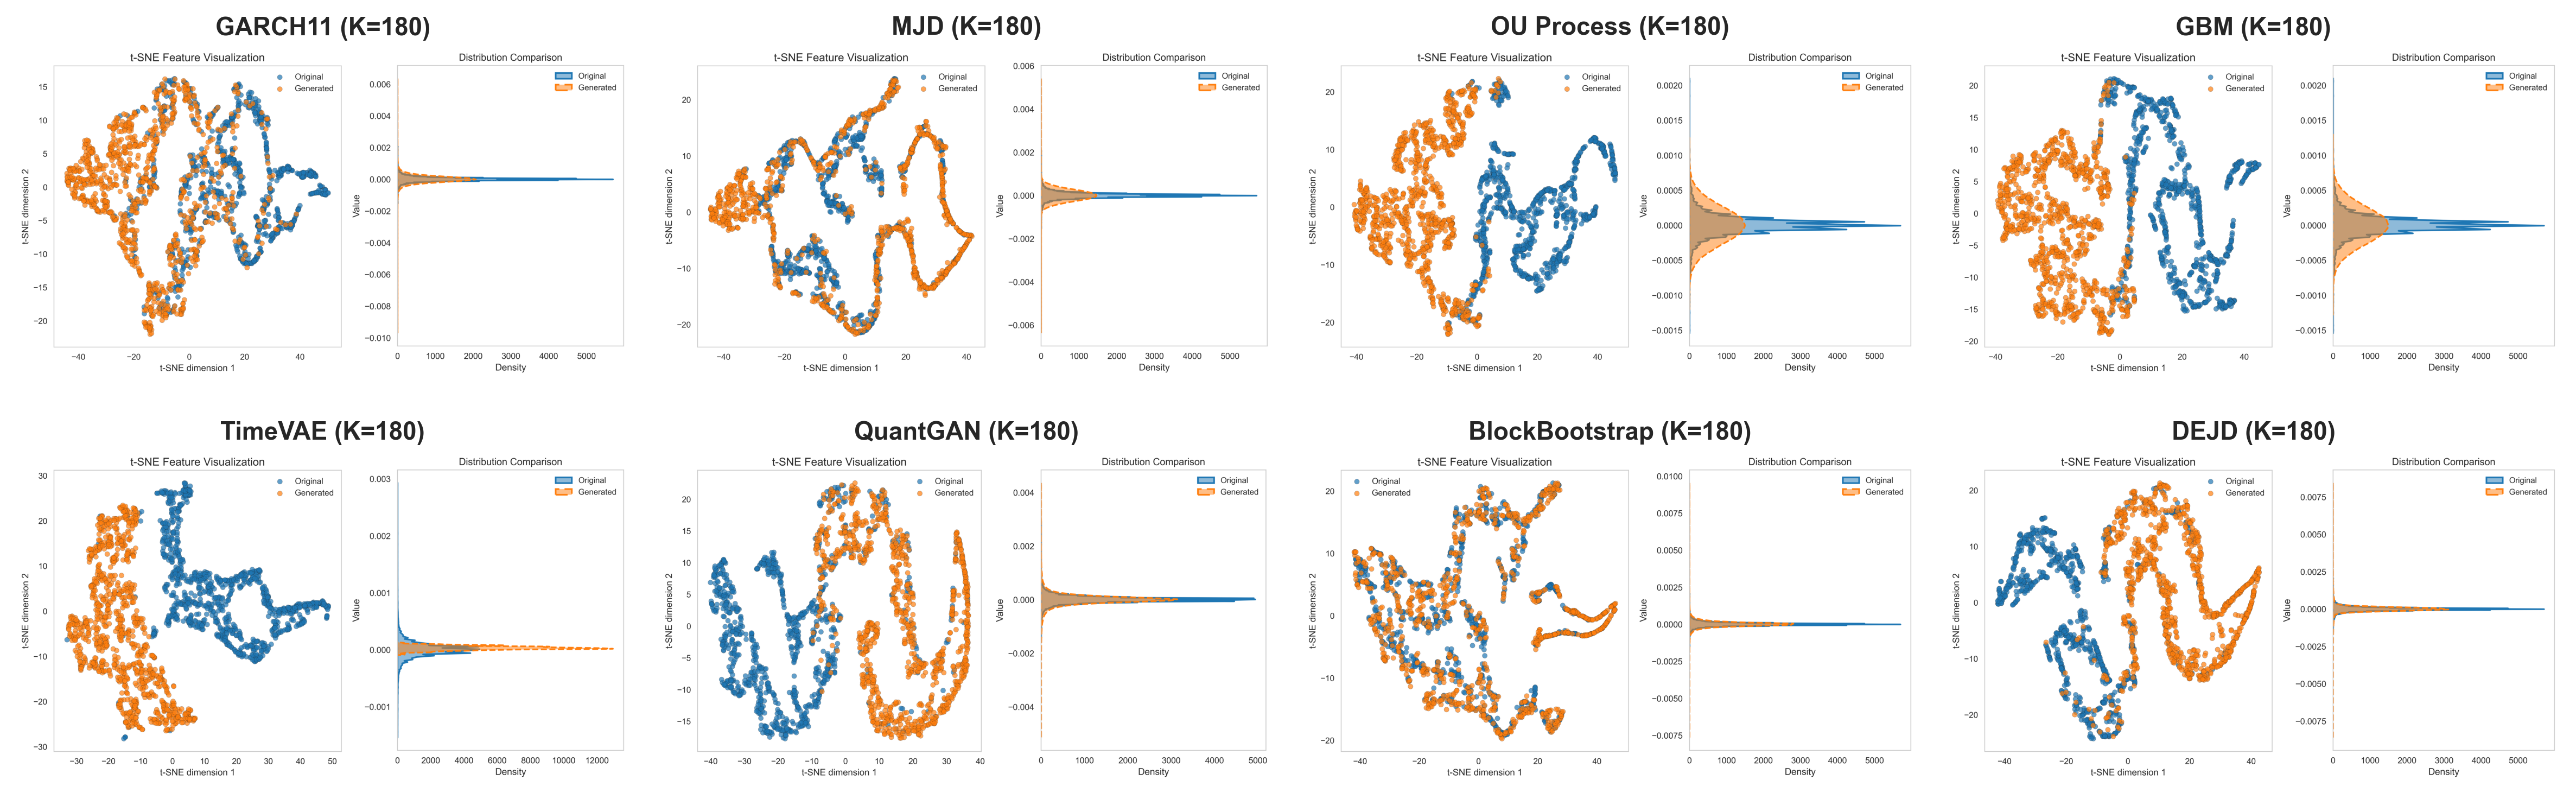
\includegraphics[width=0.9\textwidth,keepaspectratio]
  {../../results/appendix/figure_4_tsne_supplementary/figure_4_seq_180.png}
  \caption{Supplementary t-SNE visualization for sequence length 180 minutes.}
  \Description{t-SNE embeddings comparing real and synthetic data for 180-minute sequences.}
  \label{fig:tsne_seq_180}
\end{figure*}

\begin{figure*}[h]
  \centering
  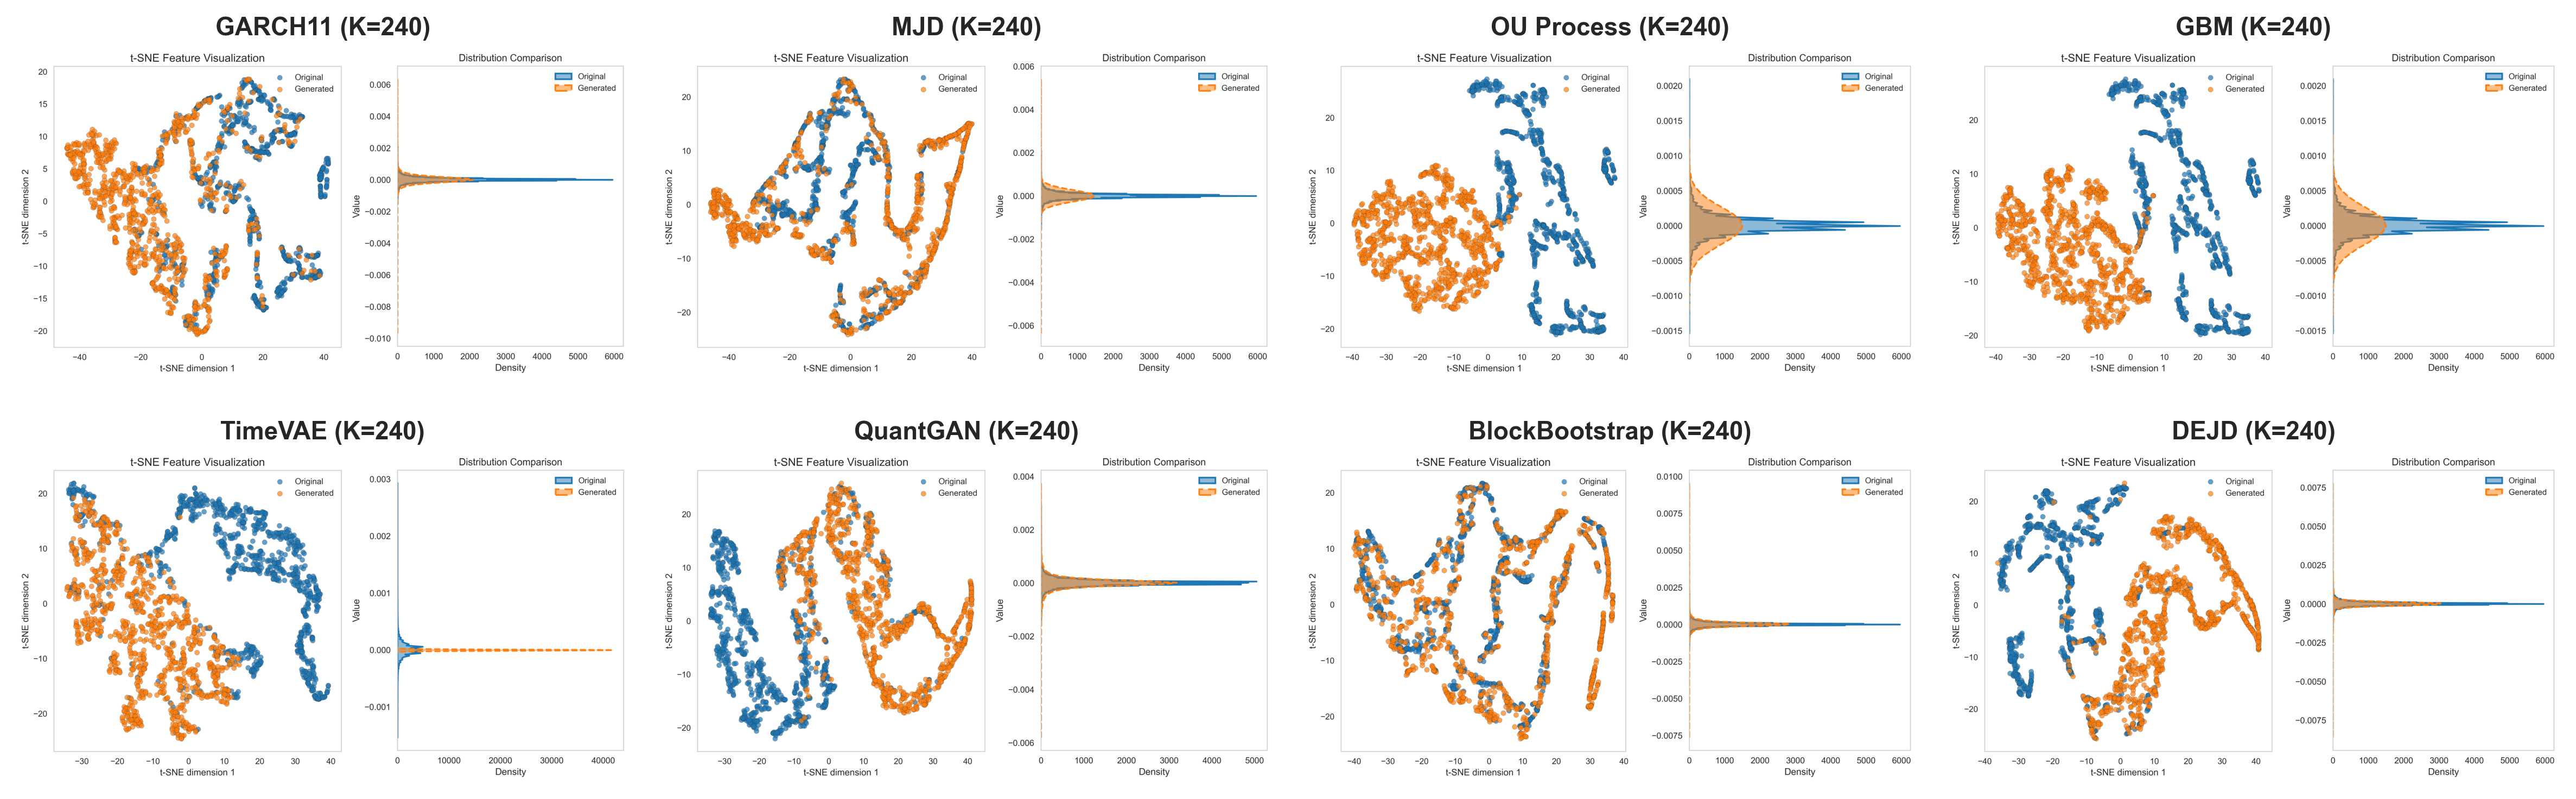
\includegraphics[width=0.9\textwidth,keepaspectratio]
  {../../results/appendix/figure_4_tsne_supplementary/figure_4_seq_240.png}
  \caption{Supplementary t-SNE visualization for sequence length 240 minutes.}
  \Description{t-SNE embeddings comparing real and synthetic data for 240-minute sequences.}
  \label{fig:tsne_seq_240}
\end{figure*}

\begin{figure*}[h]
  \centering
  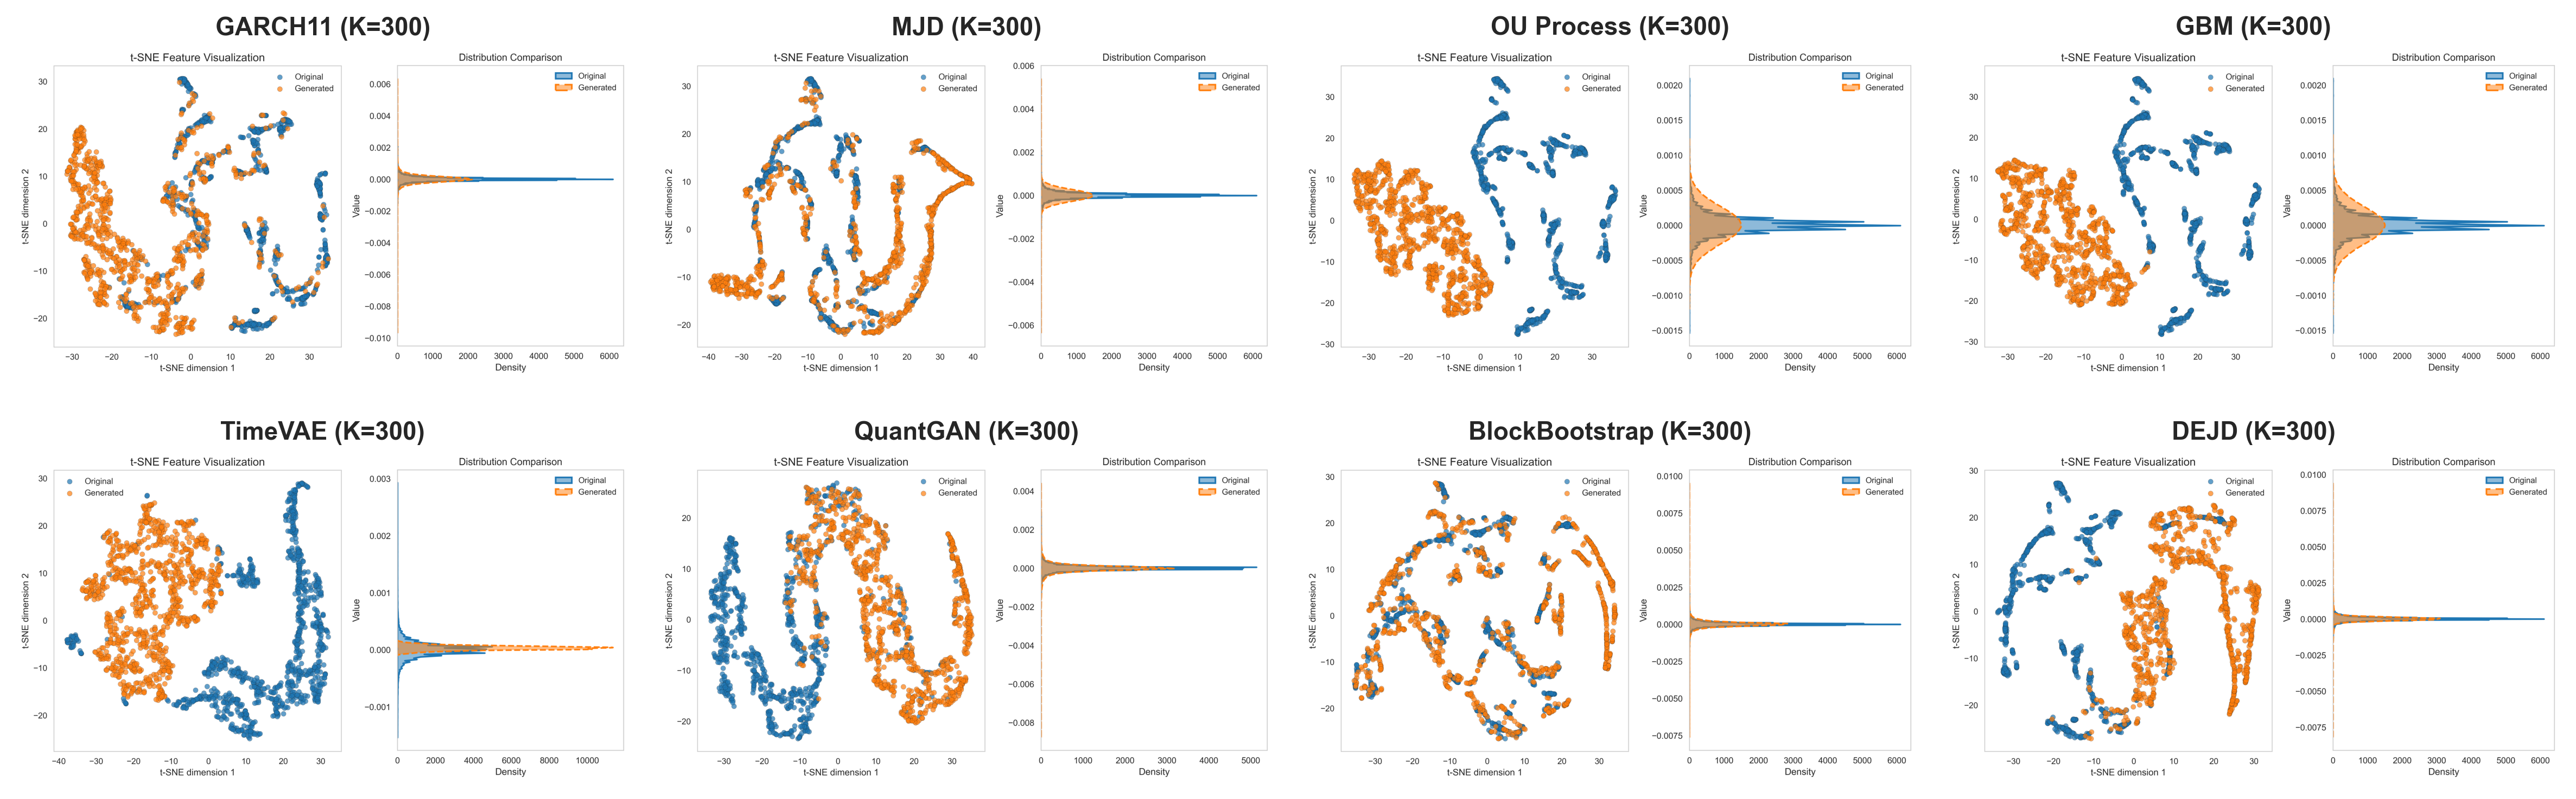
\includegraphics[width=0.9\textwidth,keepaspectratio]
  {../../results/appendix/figure_4_tsne_supplementary/figure_4_seq_300.png}
  \caption{Supplementary t-SNE visualization for sequence length 300 minutes.}
  \Description{t-SNE embeddings comparing real and synthetic data for 300-minute sequences.}
  \label{fig:tsne_seq_300}
\end{figure*}

\section{Augmented Testing Analysis}

\begin{figure*}[h]
  \centering
  
\includegraphics[width=\textwidth,keepaspectratio]
  {../../results/appendix/figure_7_augmented_testing_delta/figure_7_augmented_testing_2x4_delta.png}
  \caption{Augmented testing performance comparison showing delta metrics 
  across different hedger algorithms and SDGFTS models. Each subplot compares 
  performance when training on real data only versus augmented data 
  (real + synthetic).}
  \Description{Grid of plots showing augmented testing delta metrics for 
  different hedger models and synthetic data generators.}
  \label{fig:augmented_testing_delta}
\end{figure*}


